\chapter{深度学习的可学习性}
\label{chap:deep-learning-theory}

设一个邮件分类神经网络已经把一万封训练邮件全部分对，它有五十万个参数。第~\ref{chap:convex-learning-and-stability}章的工具会提出三个问题：训练为什么能把这样一个非凸目标降到很低；在众多同样分对训练邮件的参数中，训练最终停在哪一组；这一组参数对应的网络在新邮件上的错误率能否得到保证。三个问题都要回答，而且回答的顺序不能颠倒：先要知道训练得到什么，才能评价它的风险。

本章按这三个问题组织。第~\ref{sec:network-learning-problem}节固定研究对象：架构规定候选函数，训练算法输出其中一个，风险分解说明哪些量需要控制，并用随机标签实验说明只看架构为什么不够。第~\ref{sec:deep-training-dynamics}节研究训练本身：同一预测映射换成多层参数后，梯度更新偏向哪类解；宽网络在什么条件下近似固定核，在什么条件下特征随训练移动。第~\ref{sec:network-generalization}节把训练所得的对象接到总体风险：范数与间隔、核空间范数、样本稳定性和随机网络的PAC--Bayes代价各自需要什么条件，以及近似模型的保证怎样转回有限网络。第~\ref{sec:training-phenomena}节用这些工具审视三个具体现象：双重下降、延迟泛化和神经坍缩，区分其中已经证明的结论、可复现的观察和尚未统一的解释。

第~\ref{chap:convex-learning-and-stability}章已经建立Rademacher复杂度、稳定性和PAC--Bayes的一般结论，也在线性模型中证明了最小范数插值与最大间隔方向。本章只在需要时回顾这些结论的条件，重点放在神经网络带来的新计算：多层乘积怎样放大扰动，参数化怎样改变梯度的快慢，初始化处的梯度怎样定义特征，神经元群体怎样移动。

\section{网络学习问题}
\label{sec:network-learning-problem}

\subsection{架构、参数与训练输出}

我们先固定待分析的预测函数。神经网络的参数是训练时调整的数值，通常包括连接系数和偏置；连接系数也称为权重。以下前馈网络省略偏置，每层先用参数矩阵组合输入，再逐坐标应用激活函数，末层作线性输出。ReLU激活$\phi(a)=\max\{0,a\}$保留正值、将负值置零，多层组合因而一般不再等价于一次线性变换。将包括线性输出层在内的变换层数记为$L$，网络为
\begin{equation}
 f_{\bm W}(\bm x)=\bm W_L\phi\bigl(\bm W_{L-1}\phi(\cdots\phi(\bm W_1\bm x)\cdots)\bigr),
 \label{eq:feedforward-network}
\end{equation}
其中$\bm W_\ell\in\mathbb R^{d_\ell\times d_{\ell-1}}$，$d_0$为输入维度，$d_1,\ldots,d_{L-1}$为隐藏宽度，$d_L$为输出维度，最大宽度为$w=\max_{0\leq\ell\leq L}d_\ell$。将各层参数矩阵的元素依次排成向量$\bm\theta\in\mathbb R^p$，同一网络也记为$f_{\bm\theta}$。恢复偏置时，偏置分量也计入$\bm\theta$和参数总数$p$。

举一个具体的尺寸。邮件用$d_0=1000$个词频特征表示，经过一个宽度$d_1=500$的隐藏层后输出一个分数，即$L=2$、$d_2=1$。两层参数矩阵分别是$500\times1000$和$1\times500$，共有$p=500{,}500$个参数。训练集只有$n=10{,}000$封邮件时，参数数是样本数的五十倍。卷五以隐藏层数计量网络层数；为便于对照外部结果，本章把隐藏层数记为$L_{\mathrm h}$，总变换层数为$L=L_{\mathrm h}+1$，上例中$L_{\mathrm h}=1$。

架构、激活、宽度和深度规定网络能表示哪些函数，参数决定其中的具体函数。这两层含义不是一一对应的：同一个函数可以有许多参数表示。最简单的例子是单个ReLU单元$x\mapsto a\phi(bx)$。对任意$c>0$，$\phi(cbx)=c\phi(bx)$，因此$(a,b)$与$(a/c,cb)$给出同一个函数。图~\ref{fig:lt8-relu-rescaling}在参数平面上画出表示$x\mapsto\max\{0,x\}$的全部正参数，它们组成曲线$ab=1$。曲线上$(2,\tfrac12)$、$(1,1)$、$(\tfrac12,2)$三点的参数平方和分别是$4.25$、$2$、$4.25$，函数却完全相同；在$ab$固定时，$a^2+b^2\geq2ab$，等号只在$a=b$处成立，所以$(1,1)$是这条曲线上欧氏范数最小的表示。多层网络中，把第$\ell$层乘以$c$、第$\ell+1$层除以$c$同样不改变函数。因此，参数距离、参数范数和损失曲率的大小，都需要与“函数是否改变”分开判断；后面每次用参数量刻画网络时，都要检查它在这种重缩放下是否保持不变。

\begin{figure}[htbp]
  \centering
  % 单个ReLU单元 f(x)=a*relu(b*x) 的重缩放：(a,b) 与 (a/c, c b)（c>0）表示同一函数。
% 左：参数平面 x=a, y=b，曲线 ab=1（同一函数 x->relu(x)）；坐标 1 单位 = 14 mm。
% 三点 P1=(2,1/2)、P2=(1,1)、P3=(1/2,2)，a^2+b^2 分别为 4.25、2、4.25；
% 细圆弧 a^2+b^2=2 与曲线相切于 P2（ab 固定时 a^2+b^2>=2ab，等号当且仅当 a=b）。
% 右：三组参数对应的同一函数图像 y=relu(x)。
\begingroup
% 本图使用 specs/figures.md 的低饱和色值；以 lt8 前缀局部定义，避免覆盖共享调色板。
\definecolor{lt8Blue}{HTML}{7188A3}\definecolor{lt8BlueFill}{HTML}{E5EAF0}
\definecolor{lt8Green}{HTML}{829C8B}\definecolor{lt8GreenFill}{HTML}{E8EEE9}
\definecolor{lt8Yellow}{HTML}{B4A16F}\definecolor{lt8YellowFill}{HTML}{F1ECDD}
\definecolor{lt8Red}{HTML}{A7787D}\definecolor{lt8RedFill}{HTML}{F0E5E6}
\definecolor{lt8Ink}{HTML}{3B4252}\definecolor{lt8Muted}{HTML}{6B7280}\definecolor{lt8Stroke}{HTML}{4C4D4F}
\begin{tikzpicture}[figure picture,x=1mm,y=1mm,text=lt8Ink]
 \begin{scope}
  \draw[-{Stealth[length=1.6mm]},lt8Stroke,line width=.6pt] (0,0)--(44,0) node[right] {$a$};
  \draw[-{Stealth[length=1.6mm]},lt8Stroke,line width=.6pt] (0,0)--(0,44) node[above] {$b$};
  \node[below left] at (0,0) {$0$};
  \foreach \v/\l in {14/1,28/2}{\draw[lt8Stroke] (\v,0)--(\v,-1) node[below] {$\l$};
   \draw[lt8Stroke] (0,\v)--(-1,\v) node[left] {$\l$};}
  \draw[lt8Muted,line width=.6pt,dashed] (19.80,0) arc[start angle=0,end angle=90,radius=19.80];
  \draw[lt8Blue,line width=1.1pt,domain=0.33:2.85,samples=80,smooth] plot ({14*\x},{14/\x});
  \node[text=lt8Blue,anchor=west] at (36,9) {$ab=1$};
  \fill[lt8Red] (28,7) circle (1);  \node[anchor=south west] at (28.5,7.5) {$(2,\tfrac12)$};
  \fill[lt8Green] (14,14) circle (1.2); \node[anchor=south west] at (14.8,14.8) {$(1,1)$};
  \fill[lt8Yellow] (7,28) circle (1); \node[anchor=south west] at (7.5,28.5) {$(\tfrac12,2)$};
  \node[figure note,anchor=north] at (21,-8) {同一函数的参数集合是一条曲线};
 \end{scope}
 \begin{scope}[xshift=78mm]
  \draw[-{Stealth[length=1.6mm]},lt8Stroke,line width=.6pt] (-12,0)--(22,0) node[right] {$x$};
  \draw[-{Stealth[length=1.6mm]},lt8Stroke,line width=.6pt] (0,-2)--(0,30) node[above] {$f(x)$};
  \draw[lt8Blue,line width=1.1pt] (-11,0)--(0,0)--(20,20);
  \node[text=lt8Blue,anchor=east] at (-2,10) {$x\mapsto\max\{0,x\}$};
  \node[anchor=north west,align=left] at (3,32) {三组参数输出相同};
  \node[figure note,anchor=north] at (2,-8) {参数平方和为 $4.25$、$2$、$4.25$};
 \end{scope}
\end{tikzpicture}%
\endgroup%

  \caption{同一函数的多个参数表示。左图是单个ReLU单元$f(x)=a\max\{0,bx\}$的参数平面，蓝色曲线$ab=1$上的每一点都表示右图的函数$x\mapsto\max\{0,x\}$；三个彩色点的参数平方和分别为$4.25$、$2$、$4.25$。虚线是半径$\sqrt2$的圆，与曲线相切于$(1,1)$，说明该点是这些等价表示中欧氏范数最小的一个。参数范数因此不是函数本身的性质。}
  \label{fig:lt8-relu-rescaling}
\end{figure}

为了评价网络，取独立同分布样本$S=(z_1,\ldots,z_n)\sim\mathcal P^n$，$z_i=(\bm x_i,y_i)$。预测记为$\widehat y=f_{\bm\theta}(\bm x)$，评价预测的损失记为$\ell_{\mathrm{pred}}(\widehat y,y)$，例如分类的零一损失。把预测函数代入损失，写成$\ell_{\bm\theta}(z)=\ell_{\mathrm{pred}}(f_{\bm\theta}(\bm x),y)$，就能沿用第~\ref{sec:learning-problem}节的记号：
\[
 \hat R_S(\bm\theta)=\frac1n\sum_{i=1}^n\ell_{\bm\theta}(z_i),
 \qquad
 R_{\mathcal P}(\bm\theta)=\mathbb E_{z\sim\mathcal P}\ell_{\bm\theta}(z).
\]
分布明确时简写为$R(\bm\theta)$。讨论错误率时采用零一损失；推导梯度更新时损失须可微，届时另行写明平方损失或逻辑损失，不把优化所用的目标与最终评价的错误率混为一谈。

如果某组参数使经验风险为零，就称模型能够\term{插值}（interpolation）这份样本。插值的含义随损失而变：平方损失要求预测数值逐项等于标签；零一损失只要求类别正确；交叉熵通常要在正确类别的分数趋于无穷时才趋于零，所以类别全部分对时交叉熵仍大于零。\term{过参数化}（overparameterization）描述参数相对于样本数或拟合约束很充足的情形，常以$p>n$粗略表示。参数多只是让插值成为可能；实际能否插值，仍取决于架构、数据和损失。

研究对象于是确定为：固定数据分布、损失、架构、初始化和训练算法$A$后，算法根据样本得到的网络$A(S)$。第~\ref{sec:risk-comparison}节已经说明怎样把它的风险与候选空间$\mathcal H$中的最优风险比较。这里把那里的期望形式写成本章常用的记号：
\begin{equation}
 \begin{aligned}
 \underbrace{\mathbb E_S R(A(S))-\inf_{h\in\mathcal H}R(h)}_{\text{超额风险}}
 \leq{}&
 \underbrace{\mathbb E_S\bigl[R(A(S))-\hat R_S(A(S))\bigr]}_{\Delta_n\text{：泛化差}}\\
 &+\underbrace{\mathbb E_S\Bigl[\hat R_S(A(S))-\inf_{h\in\mathcal H}\hat R_S(h)\Bigr]}_{\rho_n\text{：经验优化误差}}.
 \end{aligned}
 \label{eq:deep-risk-decomposition}
\end{equation}
这里$\mathcal H$是所用架构表示的函数空间，相关期望假设存在；不等式成立的依据是$\mathbb E_S\inf_h\hat R_S(h)\leq\inf_hR(h)$，证明见第~\ref{sec:risk-comparison}节。若还要与所有可测预测器比较，右侧再加上近似误差$\inf_{h\in\mathcal H}R(h)-\inf_hR(h)$，它由架构的表示能力决定。三项分别对应三个问题：架构能否表示好的函数，训练是否把经验风险降到空间允许的水平，所选函数的训练表现能否代表新样本表现。训练误差下降只直接回答第二个问题；本章第~\ref{sec:deep-training-dynamics}节主要处理$\rho_n$和“选中哪个解”，第~\ref{sec:network-generalization}节处理$\Delta_n$。

\subsection{拟合能力与可学习性}

把训练标签换成随机标签，可以检验网络能否记住与输入无关的标注。Zhang等保持训练图像不变，把每张图像的类别标签独立替换为随机类别，再用相同架构和训练设置重新训练；在其部分实验中，网络仍能把训练图像全部分对\scite{zhang2021rethinking}。这里的“分对”只是复现人为指定的随机标签。由于这些标签与图像内容无关，记住它们不能帮助预测新图像的类别。

这个观察对统一的风险保证有直接的定量后果。设图像有$K$个类别，随机标签与图像独立且均匀分布，那么任何分类器在这个“随机标签分布”下的期望错误率都是$1-1/K$；实验中训练出的分类器训练错误率却为零。于是在这一样本量下，架构内至少有一个分类器的训练错误率与期望错误率相差$1-1/K$，$K=10$时为$0.9$。对所有分布同时成立的一致收敛保证必须覆盖随机标签分布，它在这一样本量下给出的差距上界就不可能小于约$0.9$。只依赖架构和样本量的保证，因而不能区分“在真实标签上训练”与“在随机标签上训练”这两种情形，而这两种情形的期望风险相差悬殊。

图~\ref{fig:learning-deep-selection}把架构、训练样本和算法的作用分开表示。架构确定可以选择哪些分类器；训练样本筛出能把当前样本全部分对的分类器；算法最终得到其中一个。以训练邮件为例，一种分类器只记住这些邮件及其标签，另一种根据词语和链接判断类别，两者都可能把训练邮件全部分对，在新邮件上却可能给出不同结果。初始化、步长、优化器或正则化也可能让算法落到不同的插值解上。只知道插值解集合有多大还不够，我们还要知道算法从中选了哪一个，以及这个解有什么可度量的性质。

\begin{figure*}[!htb]
  \centering
  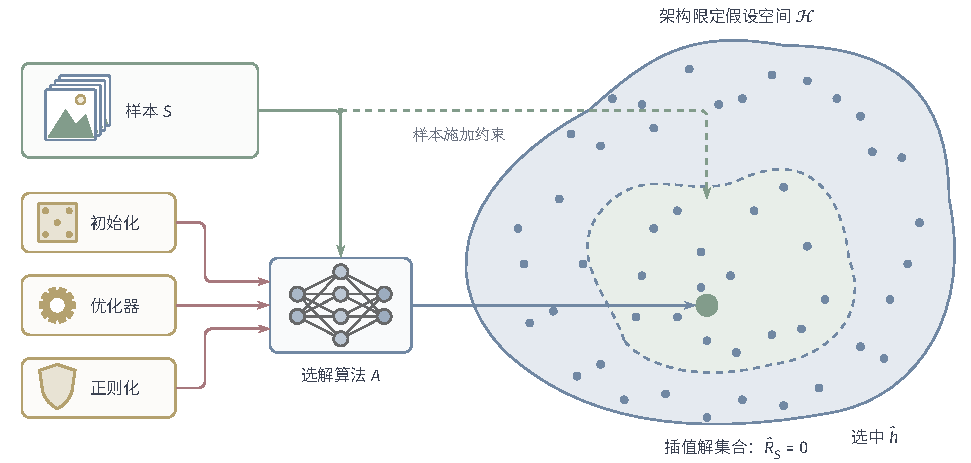
\includegraphics[width=164.600mm]{figures/06-foundations/02-learning-theory/tikz/learning-theory-deep-selection/figure.pdf}
  \caption{架构、样本和算法分别限定不同对象。外层是假设空间，内层是当前样本上经验风险为零的插值解集合；虚线表示样本施加的约束，实线表示算法的输入与输出。初始化、优化器和正则化参与选解。强调点仅示意算法选出一个插值解，不保证任意算法都实现插值；集合的形状和大小没有数值含义，插值也不保证期望风险小。}
  \label{fig:learning-deep-selection}
\end{figure*}

这并不是说架构容量没有作用。固定有限架构的VC维有限，仍可在足够样本下得到分布无关的学习保证；第~\ref{sec:network-norm-bounds}节会给出它与样本量的关系，并说明它在实际规模下为何过于宽松。随机标签实验说明的是，要解释真实标签下的泛化，还必须利用数据分布，以及训练实际选择的函数。

由此得到后文的问题顺序。第一，同一预测映射写成多层参数、换一种初始化后，梯度更新为什么会偏向不同的解；第二，宽网络在什么条件下近似一个固定特征的线性模型，什么条件下特征会随训练移动；第三，得到一个低训练误差的网络后，还需控制哪些量才能约束它的期望风险，近似模型的保证又怎样转回有限网络。训练误差已经很低以后，风险曲线、测试表现和内部表示仍可能继续变化；这些现象放在最后，作为检验前面分析工具的案例。

\section{训练动力学}
\label{sec:deep-training-dynamics}

本节只回答训练过程及其输出的性质：参数怎样运动，最终偏向哪类函数，拟合速度由什么决定。先考察参数化本身怎样改变更新和选解，再比较宽网络的两种分析模型：固定初始特征的神经切线核，以及允许神经元移动的平均场描述。两者都是在特定缩放和时间范围内成立的近似模型，并不穷尽全部训练过程，也不是同一网络必经的两个阶段。由这些性质推出风险保证的计算集中在第~\ref{sec:network-generalization}节。

\subsection{深层参数化与隐式偏置}
\label{sec:deep-implicit-bias}

第~\ref{sec:linear-implicit-bias}节在直接参数化的线性模型中证明：从零初始化的梯度下降停在最小欧氏范数插值解，可分逻辑回归的方向趋于最大间隔方向。这种由初始化、损失、参数化和更新规则共同产生、但没有显式写进目标函数的选解倾向，称为\term{隐式偏置}（implicit bias）。本节保持“同一个预测映射”这一对象，只把它写成多层参数，观察训练的运动和偏好怎样改变。

先看一个标量例子。模型$wx$直接训练$w$时，若损失对$w$的导数为$g$，每步更新都是$-\eta g$，与$w$当前的大小无关。改写成$w=uv$后，$u$的更新是$-\eta gv$，$v$的更新是$-\eta gu$，于是$w$本身的变化约为$-\eta g(u^2+v^2)$：系数已经较大时变化更快，接近零时几乎不动。两种写法表示同一族函数，训练却走出不同的路线。\term{梯度动力学}（gradient dynamics）研究这些连续更新怎样决定最终函数。下面先用可以精确求解的矩阵分解看清这种快慢差别，再研究齐次分类网络中的间隔选解，最后限定“隐式偏置”这一说法能解释什么。

\subsubsection{深层线性模型的谱动力学}

深层线性网络没有激活函数，$\bm W=\bm W_L\cdots\bm W_1$给出的仍是线性映射$\bm W\bm x$，却已经足以显示参数化怎样改变选解。典型应用是矩阵补全：$1000\times1000$的用户—电影评分矩阵只观测到约1\%的元素，满足所有观测值的矩阵有无穷多个。若用户偏好主要由题材、年代等少数因素决定，真实评分矩阵近似低秩，偏好低秩解的算法就更可能猜对未观测元素。这里要回答的问题是：把矩阵写成多个因子的乘积并用梯度训练，会不会自动偏向奇异值集中在少数方向的解。

先用二层分解$\bm W=\bm U\bm V^\top$计算这项区别。记经验目标$\mathcal L(\bm W)$及梯度$\bm G=\nabla_{\bm W}\mathcal L$，链式法则给出$\dot{\bm U}=-\bm G\bm V$、$\dot{\bm V}=-\bm G^\top\bm U$，从而
\begin{equation}
 \dot{\bm W}=-\bm G\bm V\bm V^\top-\bm U\bm U^\top\bm G.
 \label{eq:factorized-gradient-flow}
\end{equation}
直接训练$\bm W$时更新方向就是$-\bm G$；采用分解后，梯度两侧乘上了随训练变化的矩阵$\bm V\bm V^\top$和$\bm U\bm U^\top$。与标量例子$w=uv$一样，已经较强的方向更新更快，接近零的方向几乎不动。要把这一直觉变成关于奇异值的确切结论，需要一个让各层结构相互匹配的初始化条件。

平衡初始化要求相邻层满足$\bm W_{j+1}^\top\bm W_{j+1}=\bm W_j\bm W_j^\top$。在标量情形，条件变为各层系数的绝对值相等。设它们都等于$\sigma^{1/L}$且为正，端到端系数为$\sigma$，损失对$\sigma$的导数为$g$。第$j$层的更新为$\dot w_j=-g\prod_{i\neq j}w_i=-g\sigma^{(L-1)/L}$，各层更新相同，所以平衡保持；乘积的变化率为$\dot\sigma=\sum_j\bigl(\prod_{i\neq j}w_i\bigr)\dot w_j=-Lg\sigma^{2(L-1)/L}$。矩阵情形中，平衡条件要求相邻两层的奇异值相同、且第$j+1$层的右奇异向量与第$j$层的左奇异向量对齐，于是端到端矩阵在每个奇异方向上都退化为上面的标量情形。这是一个较强的简化条件；从接近零的小初始化出发时，它近似成立，一般尺度的随机初始化并不满足。

\begin{theorem}[平衡深层线性网络的梯度流]
\label{thm:balanced-deep-linear-flow}
设$L,q\geq1$，$\bm W_j(t)\in\mathbb R^{q\times q}$，
$\mathcal L:\mathbb R^{q\times q}\to\mathbb R$连续可微。记
$\bm W=\bm W_L\cdots\bm W_1$、$\bm G=\nabla\mathcal L(\bm W)$，并令各因子满足
\[
 \dot{\bm W}_j
 =-(\bm W_L\cdots\bm W_{j+1})^\top
   \bm G
   (\bm W_{j-1}\cdots\bm W_1)^\top,\qquad 1\leq j\leq L,
\]
其中空乘积为$\bm I_q$。假设初始化满足
\[
 \bm W_{j+1}(0)^\top\bm W_{j+1}(0)
 =\bm W_j(0)\bm W_j(0)^\top,\qquad 1\leq j<L.
\]
在该微分方程的解存在且各层满秩的时间区间内，平衡关系保持，且
\begin{equation}
 \dot{\bm W}
 =-\sum_{j=1}^{L}
   (\bm W\bm W^\top)^{(L-j)/L}\bm G
   (\bm W^\top\bm W)^{(j-1)/L}.
 \label{eq:balanced-matrix-gradient-flow}
\end{equation}
在某个正奇异值$\sigma_k$为单重且可微的时刻，若其左右奇异向量为$\bm u_k,\bm v_k$，则
\begin{equation}
 \dot\sigma_k=-L\sigma_k^{2-2/L}\bm u_k^\top\bm G\bm v_k.
 \label{eq:deep-singular-value-dynamics}
\end{equation}
\end{theorem}
\begin{proof}
写$\bm A_j=\bm W_L\cdots\bm W_{j+1}$、$\bm B_j=\bm W_{j-1}\cdots\bm W_1$，空乘积取单位矩阵。由乘积求导，$\dot{\bm W}=\sum_j\bm A_j\dot{\bm W}_j\bm B_j$；代入$\dot{\bm W}_j=-\bm A_j^\top\bm G\bm B_j^\top$得
\[
 \dot{\bm W}=-\sum_j\bm A_j\bm A_j^\top\bm G\bm B_j^\top\bm B_j.
\]
再检查平衡关系是否保持。由$\dot{\bm W}_{j+1}=-\bm A_{j+1}^\top\bm G\bm B_{j+1}^\top$、$\bm B_{j+1}=\bm W_j\bm B_j$与$\bm A_j=\bm A_{j+1}\bm W_{j+1}$，得
$\bm W_{j+1}^\top\dot{\bm W}_{j+1}=-\bm A_j^\top\bm G\bm B_j^\top\bm W_j^\top=\dot{\bm W}_j\bm W_j^\top$。
对其取转置并相加，即$\frac{\mathrm d}{\mathrm dt}(\bm W_{j+1}^\top\bm W_{j+1})=\frac{\mathrm d}{\mathrm dt}(\bm W_j\bm W_j^\top)$，所以两者之差恒为初值零。平衡关系允许把各层写成相互匹配的奇异值分解$\bm W_j=\bm U_j\bm D\bm U_{j-1}^\top$，其中$\bm U_j$正交、$\bm D$为同一个非负对角阵。于是$\bm W=\bm U_L\bm D^L\bm U_0^\top$，而
$\bm A_j\bm A_j^\top=\bm U_L\bm D^{2(L-j)}\bm U_L^\top=(\bm W\bm W^\top)^{(L-j)/L}$、
$\bm B_j^\top\bm B_j=\bm U_0\bm D^{2(j-1)}\bm U_0^\top=(\bm W^\top\bm W)^{(j-1)/L}$。
代回乘积导数得到第一式。单重奇异值满足$\dot\sigma_k=\bm u_k^\top\dot{\bm W}\bm v_k$；由于$\bm u_k^\top(\bm W\bm W^\top)^{(L-j)/L}=\sigma_k^{2(L-j)/L}\bm u_k^\top$且$(\bm W^\top\bm W)^{(j-1)/L}\bm v_k=\sigma_k^{2(j-1)/L}\bm v_k$，每个求和项贡献$-\sigma_k^{2-2/L}\bm u_k^\top\bm G\bm v_k$，共$L$项，得到第二式。
\end{proof}

式~\eqref{eq:deep-singular-value-dynamics}中，奇异值的变化速率含有因子$\sigma_k^{2-2/L}$。$L=1$时因子恒为1，每个方向按梯度投影匀速推进；$L\geq2$时，奇异值越小，推进越慢。取$L=3$，因子为$\sigma_k^{4/3}$：奇异值为1的方向速率因子为1，奇异值为$0.01$的方向只有约$0.01^{4/3}\approx2\times10^{-3}$。

为了看见这种快慢差别怎样随时间累积，取一个可以逐方向求解的例子。完全观测的平方损失$\mathcal L(\bm W)=\tfrac12\|\bm W-\bm W_\star\|_F^2$中，目标$\bm W_\star=\operatorname{diag}(3,1,0.3)$，各层平衡、奇异方向与$\bm W_\star$对齐，初值$\sigma_k(0)=10^{-3}$。此时$\bm G=\bm W-\bm W_\star$，对齐的奇异方向保持不变，$\bm u_k^\top\bm G\bm v_k=\sigma_k-s_k$，式~\eqref{eq:deep-singular-value-dynamics}化为三个互不耦合的标量方程
\[
 \dot\sigma_k=L\sigma_k^{2-2/L}(s_k-\sigma_k),\qquad s_k\in\{3,1,0.3\}.
\]
$L=1$时$\sigma_k(t)=s_k-(s_k-\sigma_k(0))e^{-t}$，三个方向到达目标一半的时间都约为$\ln2\approx0.69$。$L=2$时方程是逻辑方程，解为$\sigma_k(t)=s_k/\bigl(1+(s_k/\sigma_k(0)-1)e^{-2s_kt}\bigr)$，到达一半的时间约为$\ln(s_k/\sigma_k(0))/(2s_k)$，依次为$1.34$、$3.45$、$9.51$；$L=3$的数值解依次为$3.14$、$9.15$、$29.1$。图~\ref{fig:lt8-deep-linear-spectrum}画出全部九条曲线。深度增加后，每个方向从停滞到饱和的过渡变陡，不同方向的过渡时间按目标大小拉开：$L=3$时在$t=5$附近停止训练，最大方向已到达3，第二、三个方向只有约$0.008$和$0.0016$，不到各自目标的1\%，端到端矩阵近似秩一；$L=1$在同一时刻三个方向都已基本到达目标。这种“先学强方向、再学弱方向”的顺序，就是深层分解偏向低秩的机制。

\begin{figure*}[htbp]
  \centering
  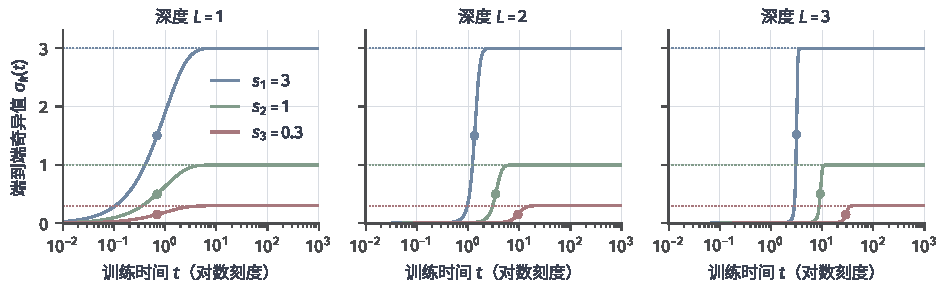
\includegraphics[width=160mm]{figures/06-foundations/02-learning-theory/matplotlib/lt8-deep-linear-spectrum/figure.pdf}
  \caption{平衡深层线性网络中各奇异值的增长。设定为完全观测平方损失$\tfrac12\|\bm W-\operatorname{diag}(3,1,0.3)\|_F^2$，各层平衡且与目标奇异方向对齐，初值$\sigma_k(0)=10^{-3}$；曲线是方程$\dot\sigma_k=L\sigma_k^{2-2/L}(s_k-\sigma_k)$的数值解，点线是目标值，圆点标出到达目标一半的时刻。横轴为对数时间。$L=1$时三个方向同时到达一半；$L=2,3$时过渡变陡，并按目标大小依次发生。该例的观测完整，只用于显示时间分离，不说明欠定观测下恢复何种矩阵。}
  \label{fig:lt8-deep-linear-spectrum}
\end{figure*}

这个例子的观测是完整的，所有方向最终都会被学到。矩阵补全或矩阵感知中的观测欠定，梯度投影$\bm u_k^\top\bm G\bm v_k$的符号和大小随训练变化，不同方向也会耦合；Arora等的理论与实验表明，在这些设定中增加分解深度会加强低秩倾向，并常常改善恢复精度\scite{arora2019deepfactorization}。因此本小节的结论限定为：深层参数化改变各谱方向的增长速度，在小初始化、近似平衡和相应观测条件下表现出低秩倾向。谱演化本身不推出矩阵恢复或低预测风险；二层因子范数与端到端核范数的静态关系，以及矩阵预测的风险定理，放在第~\ref{sec:network-norm-bounds}节连接。离散梯度下降还需控制步长与平衡误差。

\subsubsection{齐次网络的间隔选解}

矩阵分解的选解发生在插值之前的过程中：低秩是因为某些方向来不及长大。分类问题还有另一种情形：训练样本已经全部分对，逻辑损失或交叉熵仍在下降。这时训练继续改变什么，需要用分数离改判有多远来描述。

设有三个类别，真实类别为第一类。分数$(3,2,0)$与$(2.01,2,0)$都分类正确，但真实类别领先第二名的幅度分别为1和$0.01$。我们把真实类别领先其余类别的幅度称为分类间隔。

\begin{definition}[分类间隔]
\label{def:network-margin}
设$f_{\bm W}:X\to\mathbb R^K$是分类分数函数。
其在带标签输入$(\bm x,y)$处的分类间隔定义为
\begin{equation}
 \operatorname{margin}_{\bm W}(\bm x,y)
 =f_{\bm W}(\bm x)_y-\max_{j\neq y}f_{\bm W}(\bm x)_j.
 \label{eq:network-margin}
\end{equation}
对于取值为$\{-1,+1\}$的二分类标签和标量分数$f(\bm x)$，定义间隔为$yf(\bm x)$。
\end{definition}

间隔为正时，真实类别分数高于其余类别；间隔为零表示平局，后文的风险界把它计为错误。把所有分数同时乘以10，分类结果不变，间隔却放大10倍。所以原始间隔只有连同分数的尺度一起才有意义，第~\ref{sec:network-norm-bounds}节将用这一点建立风险界。

\paragraph{齐次网络与发散的参数范数}

无偏置的ReLU网络有一个关键性质。ReLU满足$\phi(cu)=c\phi(u)$（$c>0$），把式~\eqref{eq:feedforward-network}中所有$L$层参数同乘$c$，输出乘以$c^L$：$f_{c\bm\theta}(\bm x)=c^Lf_{\bm\theta}(\bm x)$。具有这一性质的模型称为$L$次正齐次的。对它，Euler恒等式$\langle\bm\theta,\nabla_{\bm\theta}f_{\bm\theta}(\bm x)\rangle=Lf_{\bm\theta}(\bm x)$在可微点成立：沿着$c\mapsto f_{c\bm\theta}$在$c=1$处求导即得。

取二分类训练样本，记第$i$个样本的间隔为$q_i(\bm\theta)=y_if_{\bm\theta}(\bm x_i)$，经验逻辑损失为$\hat R_S(\bm\theta)=n^{-1}\sum_i\log(1+e^{-q_i(\bm\theta)})$。设某一时刻所有$q_i>0$。沿着$\bm\theta\mapsto c\bm\theta$放大参数，每个$q_i$乘以$c^L$，损失严格下降并趋于零，却在任何有限参数上都取不到零。于是只要训练继续降低损失，参数范数就必须增长。梯度流$\dot{\bm\theta}=-\nabla\hat R_S(\bm\theta)$给出这一增长的精确形式：
\[
 \frac{\mathrm d}{\mathrm dt}\frac12\|\bm\theta\|_2^2
 =\Bigl\langle\bm\theta,\frac1n\sum_{i=1}^n\frac{\nabla q_i(\bm\theta)}{1+e^{q_i(\bm\theta)}}\Bigr\rangle
 =\frac Ln\sum_{i=1}^n\frac{q_i(\bm\theta)}{1+e^{q_i(\bm\theta)}}>0,
\]
第二个等号使用Euler恒等式。范数持续增长、参数本身不收敛时，有意义的对象变成参数方向$\bm\theta/\|\bm\theta\|_2$和不随整体缩放改变的归一化间隔
\[
 \bar\gamma(\bm\theta)=\frac{\min_iq_i(\bm\theta)}{\|\bm\theta\|_2^L}.
\]

第~\ref{sec:linear-implicit-bias}节的线性逻辑回归是$L=1$的特例：在那里，可分数据上的梯度下降方向收敛到最大间隔方向，这是凸问题中的全局结论。网络的情形有两处不同。一是间隔问题本身非凸：在$\|\bm\theta\|_2\leq1$上最大化$\min_iq_i(\bm\theta)$可能有多个局部最优；二是同一函数有许多参数表示，方向的极限未必唯一。所以不能把线性模型的全局结论直接照搬。

\paragraph{归一化间隔与KKT条件}

线性情形中，最大间隔问题可等价地写成在间隔约束下最小化范数。对齐次网络写出同样形式的约束优化问题：
\begin{equation}
 \min_{\bm\theta}\ \frac12\|\bm\theta\|_2^2
 \qquad\text{满足}\qquad q_i(\bm\theta)\geq1,\quad1\leq i\leq n.
 \label{eq:homogeneous-margin-problem}
\end{equation}
由齐次性，任意$\bm\theta$都可缩放成满足约束的$\bm\theta/(\min_iq_i)^{1/L}$，其范数平方为$\bar\gamma(\bm\theta)^{-2/L}$；所以最小化范数等价于最大化归一化间隔。在$q_i$光滑的点，该问题的一阶必要条件（KKT条件）为：存在$\lambda_i\geq0$，使
\[
 \bm\theta=\sum_{i=1}^n\lambda_i\nabla q_i(\bm\theta),
 \qquad \lambda_i\bigl(q_i(\bm\theta)-1\bigr)=0.
\]
第二式称为互补松弛：只有间隔恰好最小的样本才有非零系数。

梯度流的方向与这组条件有直接的对应。逻辑损失的负梯度是
\[
 -\nabla\hat R_S(\bm\theta)=\frac1n\sum_iw_i\nabla q_i(\bm\theta),\qquad w_i=\frac1{1+e^{q_i}}\approx e^{-q_i}.
\]
当范数增大时，各$q_i$按$\|\bm\theta\|_2^L$的比例增长，任意两个样本的权重比$e^{-(q_i-q_j)}$以指数速度趋于零或无穷，只有间隔最小的样本保有不可忽略的权重。因此长时间后，更新方向近似是最小间隔样本梯度的非负组合，而参数本身又沿更新方向累积，这正是KKT条件中“$\bm\theta$等于活跃约束梯度的非负组合”的形式。这段论证只说明对应关系，并非证明。

Lyu与Li把这一对应变成定理\scite{lyu2020homogeneous}。他们研究正齐次、局部Lipschitz并满足一定正则性（可以不光滑，ReLU包括在内）的网络，在逻辑损失或交叉熵下作梯度流，并假设某一时刻训练损失已降到使全部样本分对的阈值以下。在这些条件下，一个光滑化的归一化间隔随时间单调不减；参数范数趋于无穷；归一化参数$\bm\theta(t)/\|\bm\theta(t)\|_2$的每个极限点（按问题~\eqref{eq:homogeneous-margin-problem}的尺度缩放后）都是该问题的KKT点（对不光滑网络使用相应的广义梯度）；归一化间隔收敛到这个KKT点上的目标值。离散梯度下降在附加的步长与光滑性条件下有对应结论。

这一结论的范围需要精确读出。KKT点只是一阶必要条件，不一定是问题~\eqref{eq:homogeneous-margin-problem}的全局最优，所以它不说“梯度下降找到最大间隔网络”；它说明的是极限点的性质，没有断言方向本身收敛到唯一极限；它还以训练已进入全部分对的阶段为前提，不说明训练怎样到达那里。

图~\ref{fig:lt8-homogeneous-margin}用一个小例子显示这些量的实际变化。24个单位圆上的二维点按$\operatorname{sign}\cos(2\vartheta)$标注，四个象限交替，线性不可分；网络为30个单元、无偏置的两层ReLU网络（$L=2$），用逻辑损失作全批量梯度下降。第84步首次全部分对，此后范数平方从约16增长到第$3\times10^5$步的约419，最小原始间隔从$0.006$增长到约$9.7$，两者都没有收敛迹象；它们的比值即归一化间隔却在约一千步内升到$0.0228$，此后只缓慢增加到$0.0230$。真正稳定下来的是方向与归一化间隔，这与上面的结论一致。

\begin{figure*}[htbp]
  \centering
  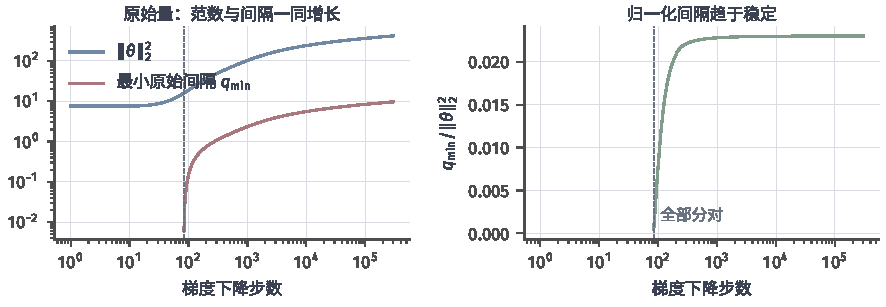
\includegraphics[width=150mm]{figures/06-foundations/02-learning-theory/matplotlib/lt8-homogeneous-margin/figure.pdf}
  \caption{齐次ReLU网络训练中的原始间隔与归一化间隔。数据为单位圆上24个点，标签为$\operatorname{sign}\cos(2\vartheta)$；网络为$f(\bm x)=\sum_{j=1}^{30}a_j\max\{0,\bm w_j^\top\bm x\}$，对参数2次齐次；逻辑损失全批量梯度下降，步长$0.2$，共$3\times10^5$步。左图双对数坐标中，参数范数平方$\|\bm\theta\|_2^2$与最小原始间隔$q_{\min}=\min_iy_if(\bm x_i)$持续增长；右图的归一化间隔$q_{\min}/\|\bm\theta\|_2^2$在全部分对（虚线）后很快趋于稳定。这是本书的合成实验，只演示所述量的变化，不检验极限点是否为全局最大间隔。}
  \label{fig:lt8-homogeneous-margin}
\end{figure*}

\subsubsection{训练偏好的解释边界}

对照两个例子可以看出，选解结论依赖参数化、初始化、损失与更新规则：矩阵分解的低秩倾向来自小初始化和乘积结构，齐次网络的间隔选解来自指数型尾部的损失和齐次性。改变其中任何一项，偏好都可能改变。两个结论首先描述训练轨迹及其极限的性质。低秩倾向或较大的归一化间隔并不自动成为风险保证；第~\ref{sec:network-generalization}节还需把它们与数据分布、尺度和有效复杂度连接起来。

一种自然的希望是把所有隐式偏置统一表述为“梯度下降在最小化某个范数”。线性回归中这确实成立；Gunasekar等也在观测矩阵两两可交换、初始化趋零及插值极限存在等条件下，把二层矩阵分解的极限与最小核范数解联系起来\scite{gunasekar2017matrix}。但Razin与Cohen构造了自然的矩阵补全问题，在其上梯度流使平方经验风险趋于零，而所有矩阵范数及拟范数都发散到无穷，同时有效秩趋于最小\scite{razin2020norms}。所以不能把隐式偏好一般地说成最小化某个范数。这个反例只限制这种一般化的解释，并不否定第~\ref{sec:linear-implicit-bias}节在特定线性模型中已经证明的最小范数结果。

\subsection{固定特征下的训练：神经切线核}
\label{sec:neural-tangent-kernel}

上一小节的结论都要求先能写出整条轨迹。非线性网络一般做不到这一点。但有一种情形可以完整求解：训练确实改变了网络的输出，参数却只在初始化附近移动了很小一段，网络在这段范围内近似是参数的线性函数。

为什么参数可能只移动一小段？设两层网络有$m$个隐藏单元，输出按$1/\sqrt m$缩放，每个参数初始化为常数量级。要让输出改变常数量级，$m$个单元共同承担这份改变，每个单元的参数只需改变约$1/\sqrt m$；单元越多，每个参数需要走的距离越短。这只是数量级的直觉，严格结论需要指定参数化、初始化与训练时长。

\paragraph{初始化处的线性化}

先固定标量输出分数（$d_L=1$）；多输出时，相应对象是带输出索引的雅可比矩阵。把输入$\bm x$映射为初始梯度$\bm\varphi_0(\bm x)=\nabla_{\bm\theta}f_{\bm\theta^{(0)}}(\bm x)$：这个向量的每个坐标记录在初始化处轻微调整某一个参数，这个输入的输出分数会改变多少。记初始函数$f_0=f_{\bm\theta^{(0)}}$，一阶展开为
\begin{equation}
 f_{\bm\theta}(\bm x)\approx
 f_0(\bm x)+\langle\bm\varphi_0(\bm x),\bm v\rangle,
 \qquad \bm v=\bm\theta-\bm\theta^{(0)}.
 \label{eq:initial-gradient-feature-map}
\end{equation}
它把参数位移映射为函数增量：线性化模型中可训练的量是位移$\bm v$，特征$\bm\varphi_0$保持不动。以图~\ref{fig:learning-ntk-linearization}中的两参数网络$f_{(a,b)}(x)=a\tanh(bx)$为例，初值取$(a,b)=(1,1)$，对参数求导得$\bm\varphi_0(x)=(\tanh x,\ x\operatorname{sech}^2x)^\top$，于是$\bm\varphi_0(1)\approx(0.76,0.42)^\top$，$\bm\varphi_0(2)\approx(0.96,0.14)^\top$。在$x=2$处$\tanh$已接近饱和，调整$b$的作用小得多，所以第二个坐标只有$0.14$。图中沿实际训练轨迹比较真实输出与一阶近似，几步训练内二者几乎重合，余项很小但并非零。

\begin{figure*}[!htb]
  \centering
  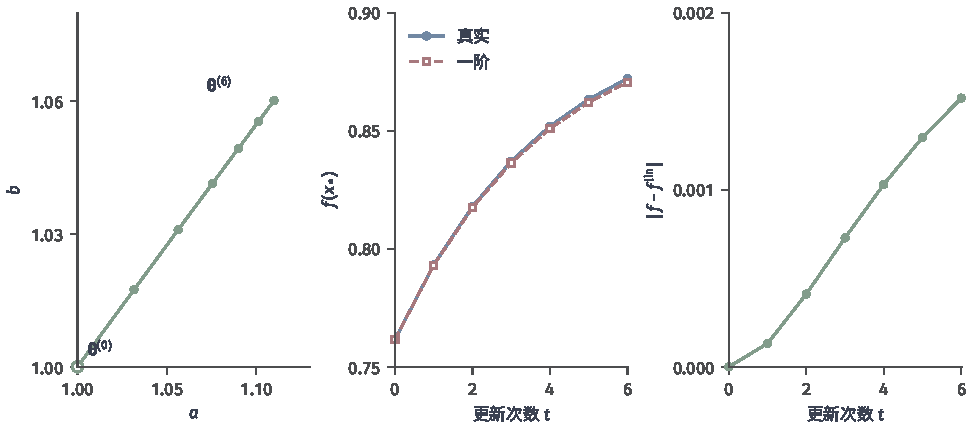
\includegraphics[width=164.600mm]{figures/06-foundations/02-learning-theory/matplotlib/learning-theory-ntk-linearization/figure.pdf}
  \caption{初始化附近的参数轨迹与输出线性化。教学网络为$f_{(a,b)}(x)=a\tanh(bx)$，初值为$(1,1)^\top$；用单个样本$(x,y)=(1,0.9)$的半平方损失、步长$0.3$执行六次梯度下降，连同初值共七个检查点。中间的真实输出和一阶输出均在左侧同一参数轨迹上计算；三面板各用所标坐标范围，不能按纸面高度直接比较数值。右侧余项末次约为$0.00152$。参数增量经初始雅可比映射到输出空间的切空间。此有限网络示例展示近似对象，不证明训练中核恒定或新输入上的误差受控。}
  \label{fig:learning-ntk-linearization}
\end{figure*}

在线性化模型中，从$\bm v=0$开始，每次经验风险梯度都是训练样本处初始梯度特征的线性组合，所以参数更新始终落在$\operatorname{span}\{\bm\varphi_0(\bm x_1),\ldots,\bm\varphi_0(\bm x_n)\}$内。新输入的特征可以不在这个子空间，但它与训练样本特征的内积决定所学更新怎样影响预测。为表达这一传递关系，我们定义梯度内积对应的核。

\begin{definition}[神经切线核]
\label{def:neural-tangent-kernel}
设网络输出对参数可微。参数为$\bm\theta$时的\term{神经切线核}（neural tangent kernel, NTK）为
\[
 K_{\bm\theta}(\bm x,\bm x')=
 \left\langle\nabla_{\bm\theta}f_{\bm\theta}(\bm x),
               \nabla_{\bm\theta}f_{\bm\theta}(\bm x')\right\rangle.
\]
记$K_0=K_{\bm\theta^{(0)}}$，其在训练输入上的核矩阵为$\bm K_0$，$(\bm K_0)_{i,j}=K_0(\bm x_i,\bm x_j)$。
\end{definition}

核由架构、初始化及输出缩放共同决定。它直接给出一次更新怎样传播：若用第$i$个训练样本更新，损失对当前分数的导数为$a_i$，在线性化模型中$\Delta\bm v=-\eta a_i\bm\varphi_0(\bm x_i)$，于是$\Delta f(\bm x_j)=-\eta a_iK_0(\bm x_j,\bm x_i)$。沿用上面的例子，$K_0(1,1)\approx0.76$，$K_0(1,2)\approx0.79$；在$x=1$处做一次使输出升高$0.1$的更新，$x=2$处的输出也升高约$0.1\times0.79/0.76\approx0.10$。图~\ref{fig:learning-ntk-features}把这次更新分成两步：训练样本处的损失梯度产生参数增量，另一输入处的输出梯度把增量转换为预测变化。

\begin{figure*}[!htb]
  \centering
  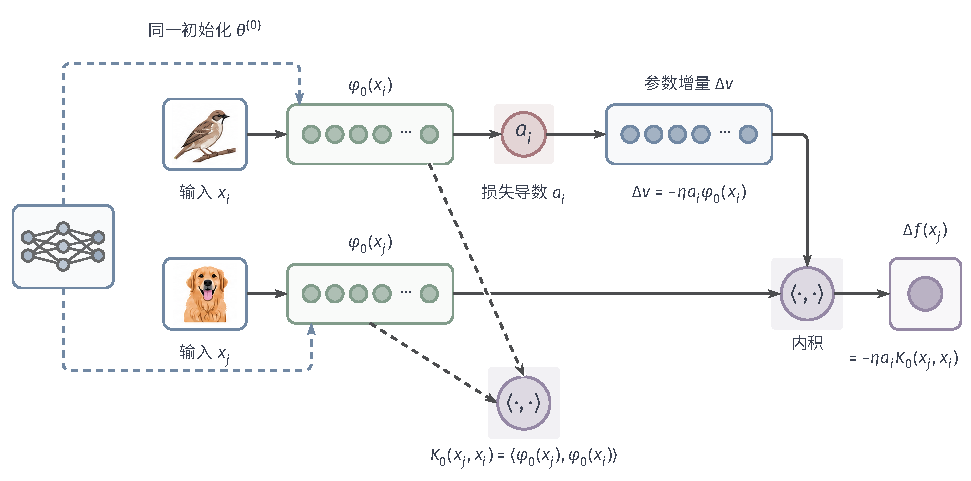
\includegraphics[width=164.600mm]{figures/06-foundations/02-learning-theory/tikz/learning-theory-ntk-features/figure.pdf}
  \caption{初始梯度特征如何传递一次训练更新。在线性化模型中，第$i$个训练样本的初始梯度特征与损失对预测的导数$a_i$共同确定参数增量$\Delta\bm v$；将同一增量与输入$\bm x_j$处的初始梯度特征作内积，得到$\Delta f(\bm x_j)$。核值$K_0$正是两个初始梯度特征的内积。特征条仅示意梯度坐标，不限定参数维数。对真实有限宽网络使用固定特征，还需控制核变化与线性化误差。}
  \label{fig:learning-ntk-features}
\end{figure*}

\paragraph{训练点上的预测动力学}

用半平方损失$\frac1{2n}\sum_i(f_i-y_i)^2$计算训练点预测值的变化，其中$\bm f(t)$和$\bm y$是训练样本上的预测与标签向量。梯度流下$\dot{\bm\theta}=-\frac1n\sum_i(f_i-y_i)\nabla_{\bm\theta}f_i$，第$j$个预测的变化率为$\dot f_j=\langle\nabla_{\bm\theta}f_j,\dot{\bm\theta}\rangle$，写成向量形式就是真实网络的梯度流
\[
 \dot{\bm f}(t)=-\frac1n\bm K_{\bm\theta(t)}(\bm f(t)-\bm y).
\]
这一式子是精确的，核随时间变化。固定核模型把$\bm K_{\bm\theta(t)}$换成$\bm K_0$。这里需要区分三个不同的陈述：一阶展开式~\eqref{eq:initial-gradient-feature-map}只是初始化处的局部近似；宽度趋于无穷时初始核收敛到确定的极限核，是关于初始化分布的陈述；训练期间核不显著漂移，是关于整段轨迹的陈述。Jacot等在特定参数化、初始化与无限宽极限下得到确定核，并证明在相应训练条件下它在训练中保持不变\scite{jacot2018ntk}。网络由固定梯度特征描述的训练称为\term{惰性训练}（lazy training）。仅凭泰勒展开，不能假定整个训练过程都满足固定核模型。

\begin{theorem}[固定NTK下的训练收敛]
\label{thm:ntk-training-convergence}
设$n\geq1$，$\bm K_0\in\mathbb R^{n\times n}$为正定矩阵，
最小特征值为$\lambda_{\min}>0$，并给定
$\bm y,\bm f(0)\in\mathbb R^n$。若
$\dot{\bm f}(t)=-\bm K_0(\bm f(t)-\bm y)/n$，则
\[
 \bm f(t)-\bm y=e^{-\bm K_0t/n}(\bm f(0)-\bm y),
\]
并有
$\|\bm f(t)-\bm y\|_2\leq e^{-\lambda_{\min}t/n}\|\bm f(0)-\bm y\|_2$。
\end{theorem}
\begin{proof}
将$\bm K_0$正交对角化为$\bm K_0=\sum_j\lambda_j\bm u_j\bm u_j^\top$，记残差分量$e_j(t)=\bm u_j^\top(\bm f(t)-\bm y)$。由于$\bm y$不随时间变化，$\dot e_j=\bm u_j^\top\dot{\bm f}=-\lambda_je_j/n$，所以$e_j(t)=e^{-\lambda_jt/n}e_j(0)$。合并各方向即得矩阵指数表达式；再由$\|\bm f(t)-\bm y\|_2^2=\sum_je^{-2\lambda_jt/n}e_j(0)^2$和$\lambda_j\geq\lambda_{\min}$控制欧氏范数。
\end{proof}

残差在核矩阵各特征向量方向上的分量，按相应特征值决定的速率衰减：大特征值方向学得快，小特征值方向学得慢，最小特征值控制最慢的方向。初始化处$f_0$一般不为零，这里的残差是相对于标签的$\bm f-\bm y$，其初值就是标签减初始预测的相反数。离散梯度下降$\bm\theta^{(t+1)}=\bm\theta^{(t)}-\eta\nabla\hat R_S$对应的固定核递推是$\bm r^{(t+1)}=(\bm I-\eta\bm K_0/n)\bm r^{(t)}$，步长须满足$\eta<2n/\lambda_{\max}$，各分量每步乘以$1-\eta\lambda_j/n$。

图~\ref{fig:lt8-ntk-residual}在一个有限网络上比较这一预测与实际训练。20个输入取在圆上，标签含两个频率，两层ReLU网络按$1/\sqrt m$缩放输出、两层都训练，步长取$n/(2\lambda_{\max})$。宽度$m=10^5$时，$\bm K_0$的特征值从约10.4下降到约$0.018$；训练3000步后，第二大特征值（约4.0）方向的残差已降到初值的约$2\times10^{-5}$，居中方向（约$0.039$）降到约$1.0\%$，固定核预测为$0.38\%$，最小方向（约$0.018$）只降到约20\%，固定核预测为$7.5\%$。快方向的拟合主要在前几十步完成，慢方向则拖着整个残差。左图中宽度越大，网络的残差曲线越接近固定核的虚线；右图显示训练结束时核的相对漂移随宽度减小，从$m=30$的约$1.1$降到$m=10^5$的约$0.004$。

\begin{figure*}[htbp]
  \centering
  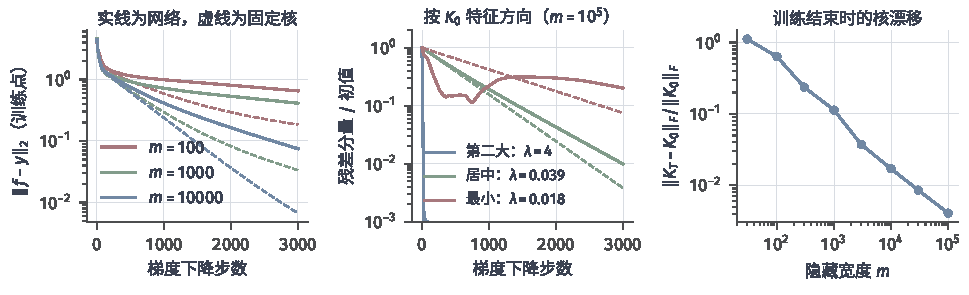
\includegraphics[width=164mm]{figures/06-foundations/02-learning-theory/matplotlib/lt8-ntk-residual/figure.pdf}
  \caption{固定核预测与有限网络训练。输入$\bm x_i=(\cos t_i,\sin t_i,1)/\sqrt2$，$t_i=2\pi i/20+0.1$，标签$y_i=\sin2t_i+\tfrac12\cos5t_i$；网络$f(\bm x)=m^{-1/2}\sum_ja_j\max\{0,\bm w_j^\top\bm x\}$，$a_j$与$\bm w_j$取标准高斯初值，半平方损失全批量梯度下降，步长$n/(2\lambda_{\max}(\bm K_0))$，3000步。左：训练残差范数，实线为网络，虚线为以初始核$\bm K_0$递推的固定核模型。中：$m=10^5$时残差在$\bm K_0$三个特征方向上的分量与初值之比，虚线为$(1-\eta\lambda/n)^t$。右：训练结束时核的相对Frobenius漂移。每个宽度一次运行，随机种子记录在图源中。}
  \label{fig:lt8-ntk-residual}
\end{figure*}

正定性来自哪里也值得说明。$\bm K_0$是$n$个梯度特征的Gram矩阵，正定等价于这些特征线性无关，必要条件是$p\geq n$。过参数化在这里起到正面作用：它使线性化模型有可能插值全部训练样本，这是非凸训练仍能把损失降到零的一种解释。但核矩阵可逆或训练损失收敛只说明训练样本上的拟合；插值所得函数的大小及其预测风险，要到第~\ref{sec:ntk-rkhs-generalization}节计算。

\subsection{变化特征下的训练：平均场模型}
\label{sec:mean-field}

固定核模型把特征冻结在初始化处，而网络相对于固定核方法的优势，常被认为恰恰来自训练中学到的特征。要描述特征怎样移动，又不必逐个追踪成千上万个神经元，平均场方法不再区分“第$j$个单元”，而是记录参数空间中每处有多少单元。

取$m$个隐藏单元的两层网络，对每个单元的贡献乘$1/m$：
\[
 f_m(\bm x)=\frac1m\sum_{j=1}^m a_j\phi(\bm w_j^\top\bm x).
\]
给每个单元参数$\bm\vartheta_j=(a_j,\bm w_j)$赋质量$1/m$，得到经验分布$\rho_m=m^{-1}\sum_j\delta_{\bm\vartheta_j}$，其中$\delta_{\bm\vartheta}$是$\bm\vartheta$处的点质量。记单元输出$\psi_{\bm\vartheta}(\bm x)=a\phi(\bm w^\top\bm x)$，求和便等于积分
\begin{equation}
 f_{\rho_m}(\bm x)=\int \psi_{\bm\vartheta}(\bm x)\,\mathrm d\rho_m(\bm\vartheta).
 \label{eq:mean-field-network}
\end{equation}
例如四个单元中两个取$(1,\bm w_1)$、两个取$(-1,\bm w_2)$，$\rho_4$在这两点上各有质量$\tfrac12$，输出为$\tfrac12\phi(\bm w_1^\top\bm x)-\tfrac12\phi(\bm w_2^\top\bm x)$；把每个单元复制成一百份，宽度变为400，分布和输出都不变。$1/m$缩放正是为了让宽度改变时输出保持在同一尺度上。

再看有限网络的梯度怎样诱导分布变化。对平方损失
\[
 \hat R_S(\rho)=\frac1{2n}\sum_i(f_\rho(\bm x_i)-y_i)^2,
\]
第$j$个单元参数的梯度为
\[
 \nabla_{\bm\vartheta_j}\hat R_S
 =\frac1m\cdot\frac1n\sum_{i=1}^n\bigl(f_{\rho_m}(\bm x_i)-y_i\bigr)\nabla_{\bm\vartheta}\psi_{\bm\vartheta_j}(\bm x_i)
 =\frac1m\nabla_{\bm\vartheta}V(\bm\vartheta_j;\rho_m),
\]
其中$V(\bm\vartheta;\rho)=\frac1n\sum_i(f_\rho(\bm x_i)-y_i)\psi_{\bm\vartheta}(\bm x_i)$。每个单元的梯度都带一个$1/m$；若步长取$\eta=m\eta'$，更新化为$\bm\vartheta_j\leftarrow\bm\vartheta_j-\eta'\nabla_{\bm\vartheta}V(\bm\vartheta_j;\rho_m)$，每个单元按同一个势函数$V(\cdot;\rho_m)$的梯度移动，而势函数又由全体单元的分布决定。所以有限网络的训练等价于一群相互作用的粒子在参数空间中运动；宽度$m\to\infty$时，$\rho_m$趋近连续分布$\rho_t$，粒子运动变成分布的演化方程$\partial_t\rho_t=\nabla_{\bm\vartheta}\cdot(\rho_t\nabla_{\bm\vartheta}V(\bm\vartheta;\rho_t))$。\term{平均场理论}（mean-field theory）研究这一极限及有限宽网络与它的距离；Mei等给出了两层网络的这一极限及有限宽近似\scite{mei2018meanfield,mei2019meanfield}。

与固定核相比，关键差别在于每个单元走多远。在$1/\sqrt m$缩放下，$m$个单元分摊一次输出改变，每个参数只需移动约$1/\sqrt m$；在$1/m$缩放下，每个单元对输出的贡献已被压到$1/m$，要让输出改变常数量级，单元参数本身就要移动常数量级，特征因而随训练改变。图~\ref{fig:lt8-mean-field-particles}用同一个学生网络和同一组初值比较两种缩放：教师函数是两个ReLU单元之和，教师方向用绿色箭头表示。$1/\sqrt m$缩放下，400个单元的输入权重平均只移动约$0.13$，分布形状几乎不变；$1/m$缩放下平均移动约$1.0$，输出权重为正的单元沿两个教师方向聚成两束。两者都把训练损失降到很低，得到的却是不同的网络。

\begin{figure*}[htbp]
  \centering
  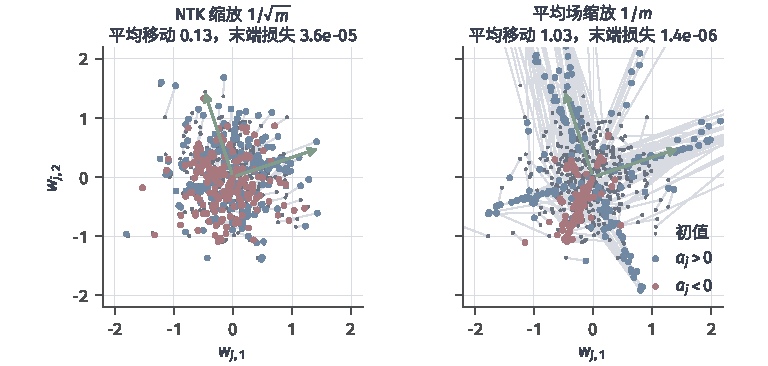
\includegraphics[width=130mm]{figures/06-foundations/02-learning-theory/matplotlib/lt8-mean-field-particles/figure.pdf}
  \caption{两种输出缩放下隐藏单元参数的移动。输入为60个标准高斯二维点，教师函数$y=\max\{0,\bm u_1^\top\bm x\}+\max\{0,\bm u_2^\top\bm x\}$，绿色箭头为$\bm u_1=(1.5,0.5)$、$\bm u_2=(-0.5,1.5)$。学生网络有$m=400$个单元，初值$\bm w_j\sim\mathcal N(0,0.25\bm I)$、$a_j\sim\mathcal N(0,1)$，两层都训练，半平方损失全批量梯度下降4000步；左图输出乘$m^{-1/2}$、步长$0.2$，右图输出乘$m^{-1}$、步长$0.2m$。灰点为$\bm w_j$初值，彩点为末值，颜色区分$a_j$末值的符号，细线连接同一单元的初值与末值。标题给出平均移动距离与末端训练损失。本书合成实验。}
  \label{fig:lt8-mean-field-particles}
\end{figure*}

固定核与平均场是两种不同的无限宽极限，取决于参数随宽度的缩放方式与训练时间，不能按“宽网络”和“窄网络”来划分：同一宽度下，换一种初始化或输出缩放，就可能从一种描述转到另一种。

还需说明分布在这里表示什么。$\rho$是组成一个网络的神经元分布，从$\rho$抽一次只得到一个单元，要经式~\eqref{eq:mean-field-network}的积分才得到确定的预测函数$f_\rho$；它不是从完整网络中随机抽取预测器的后验分布。积分对$\rho$是线性的，所以预测损失为凸函数时，风险作为$\rho$的函数也是凸的。但有限宽网络只能移动有限个质量点，在有限点上优化仍可能非凸；分布上的凸性不直接保证梯度下降在有限网络上找到全局最优。积分表示本身也不证明训练收敛，更不证明替换一个样本后分布变化很小；分布变化如何转化为输出和损失差，在第~\ref{sec:network-generalization}节的稳定性应用中处理。

\subsection{有限宽度下的近似条件}

前两小节的结论都描述某个极限或近似模型，用于有限网络时需要逐项检查近似误差控制的是什么。

初始化尺度与输出缩放决定处于哪种描述：$1/\sqrt m$缩放配合常数量级初值倾向固定核，$1/m$缩放倾向特征移动；把输出整体乘以一个较大的常数也会使所需参数位移变小，从而更接近固定核描述。宽度控制近似的精度：图~\ref{fig:lt8-ntk-residual}中核的相对漂移随宽度增加而减小。训练时间决定近似成立的区间：固定核的结论通常在给定的时间区间内成立，训练越久，参数位移越大，核漂移越可能累积。参数位移与核漂移是可以在训练中直接测量的诊断量。还需明确近似误差控制的是哪些输入：训练点上的核矩阵漂移小，不等于新输入上的线性化误差小。

近似误差的大小必须与它影响的谱方向比较。由Weyl不等式，对称矩阵的每个特征值在扰动下至多移动扰动的谱范数，而谱范数不超过Frobenius范数。图~\ref{fig:lt8-ntk-residual}的$m=10^5$运行中，核的相对漂移约$0.4\%$，按$\|\bm K_0\|_F\approx11.9$折算，绝对漂移约$0.05$，已经超过最小特征值$0.018$。所以“核几乎不变”在相对意义上成立，却保护不了最小特征值附近的方向；中图最小方向的残差偏离虚线，正是这一点的表现。固定核描述适用时，可以分析大特征值方向的残差收缩；用于小特征值方向或出现显著特征变化时，不能继续把初始核当成未经检验的全程描述。

两类分析保留的信息不同。固定核模型是线性的，便于计算拟合速度和插值解，代价是排除了特征学习；神经元分布能够描述特征移动，代价是演化方程非线性，收敛与选解都更难分析。训练轨迹被某个近似模型描述以后，还有另一个问题：近似模型的风险保证能否传给有限网络。这需要在新输入上控制两者的输出差，放到第~\ref{sec:network-generalization}节末完成。

\section{泛化保证}
\label{sec:network-generalization}

上一节说明了训练可能得到什么：低秩倾向的矩阵、较大归一化间隔的方向、固定核下的插值函数、移动后的神经元分布。本节把这些对象接到总体风险，也就是控制式~\eqref{eq:deep-risk-decomposition}中的泛化差$\Delta_n$。先从架构容量和范数约束评价网络函数空间，再把训练所得的矩阵与核插值解接入复杂度计算；随后讨论样本稳定性与随机网络的PAC--Bayes保证；最后处理近似模型到有限网络的风险转移。每条路线都会说明使用了第~\ref{chap:convex-learning-and-stability}章的哪个工具，网络结构增加了哪些计算，以及还要求训练算法满足什么条件。

\subsection{函数复杂度界}
\label{sec:network-norm-bounds}

函数复杂度路线对一个预先规定的函数集合同时控制经验风险与总体风险的偏差，因此无论训练选中集合中的哪个函数都有保证。各个界的区别在于集合从哪里得到约束：只用架构，用参数范数与分类间隔，或用训练所得函数的范数。

\subsubsection{架构容量的基线保证}

固定架构后，先估计它所表示的二分类假设空间的VC维，再代入第~\ref{sec:binary-learnability-characterization}节的学习定理。Baum与Haussler在1988年研究了阈值网络规模与泛化样本数的关系\scite{baum1988size}。估计网络的VC维时，不仅要看参数个数，还要看连接方式、层数和激活函数：平面上的线性阈值单元有3个参数，VC维恰为3，但这种巧合在网络中不再成立。对分段线性网络，Bartlett等给出ReLU网络$O(pL\log p)$的VC维上界，并在相应参数范围内构造了达到$\Omega(pL\log(p/L))$的架构\scite{bartlett2019vc}；该下界只说明存在某些架构达到这样的VC维，不适用于每个含$p$个参数的架构。

有了VC维上界，二分类学习基本定理直接给出不可知PAC形式的样本量条件。下面单独写出这一步，并保留“存在一个算法能达到该保证”与“实际优化算法能否找到对应参数”之间的区别。

\begin{theorem}[有限VC维网络的不可知PAC样本量保证]
\label{thm:network-vc-pac}
设$(X,\mathcal X)$为可测输入空间，$Y=\{0,1\}$，
$Z=X\times Y$取乘积$\sigma$代数。固定网络架构所表示的非空二分类假设空间
$\mathcal H\subseteq Y^X$由可测函数组成，其VC维为有限数$d\geq1$。
对$Z$上的任意概率分布$\mathcal P$，令
$S=((x_1,y_1),\ldots,(x_n,y_n))\sim\mathcal P^n$，并定义零一损失下的
\[
 R_{\mathcal P}(h)=\mathbb P_{(x,y)\sim\mathcal P}\{h(x)\neq y\},
 \qquad
 \hat R_S(h)=\frac1n\sum_{i=1}^n\mathbb I\{h(x_i)\neq y_i\}.
\]
假设随机变量
$\sup_{h\in\mathcal H}|\hat R_S(h)-R_{\mathcal P}(h)|$可测。
存在通用常数$c>0$，使得任意$\varepsilon,\delta\in(0,1)$和任意
$\mathcal P$下，只要
\[
 n\geq c\frac{d\log(2/\varepsilon)+\log(2/\delta)}{\varepsilon^2},
\]
每个满足$\hat R_S(\hat h)=\inf_{h\in\mathcal H}\hat R_S(h)$的经验风险
最小化算法输出$\hat h$都以至少$1-\delta$的概率满足
\[
 R_{\mathcal P}(\hat h)\leq\inf_{h\in\mathcal H}R_{\mathcal P}(h)+\varepsilon.
\]
\end{theorem}
\begin{proof}
由定理~\ref{thm:vc-uniform-convergence}，在所给样本量下（适当选取$c$），事件
\[
 \sup_{h\in\mathcal H}|\hat R_S(h)-R_{\mathcal P}(h)|\leq\varepsilon/2
\]
以至少$1-\delta$的概率成立。在该事件上，对任意$h\in\mathcal H$有
\[
 R_{\mathcal P}(\hat h)
 \leq\hat R_S(\hat h)+\frac\varepsilon2
 \leq\hat R_S(h)+\frac\varepsilon2
 \leq R_{\mathcal P}(h)+\varepsilon.
\]
对右侧的$h$取下确界即可。证明只用了ERM的经验风险比较性质，没有给出实现ERM的计算方法；训练若只实现近似ERM，还须按第~\ref{sec:risk-comparison}节计入经验优化误差。
\end{proof}

把数代进去，可以看出这条保证对大型网络意味着什么。忽略常数$c$，取$\varepsilon=0.1$、$\delta=0.05$：VC维$d=100$时右侧约为$(100\log20+\log40)/0.01\approx3\times10^4$；若把邮件网络的VC维粗略取为参数数$d\approx5\times10^5$，右侧约为$5\times10^5\times3.0/0.01\approx1.5\times10^8$，是手头一万封邮件的一万五千倍。反过来固定$n=10^4$，即使取$\varepsilon$接近1，右侧仍约为$5\times10^5\log2\approx3.5\times10^5$，在$(0,1)$中找不到满足条件的精度。这不等于更少样本一定无法学习，只说明按整个架构计算的保证在这里派不上用场。

回看第~\ref{sec:network-learning-problem}节的随机标签对照，这种宽松并非常数不够精细所致：同一架构的统一保证必须同时覆盖真实标签和随机标签，因而不会区分两个训练输出。下面引入的参数尺度、间隔和训练所得函数的约束，是补充保证所使用的额外信息，不是对容量分析的否定。

\subsubsection{间隔、尺度与输出扰动}

最直接的额外信息是参数的数值大小。考虑两个参数个数相同的线性分类器$\bm w^\top\bm x$，一个取$\bm w=(1,1)^\top$，另一个取$\bm w=(100,-99)^\top$。输入从$(1,1)^\top$变成$(1.01,1)^\top$时，前者的分数只改变$0.01$，后者却改变1。由Cauchy--Schwarz不等式$|\langle\bm w,\bm x-\bm x'\rangle|\leq\|\bm w\|_2\|\bm x-\bm x'\|_2$，范数正好记录这种放大能力：两者的范数约为$1.41$和$140.7$。Bartlett在1996年研究了适当条件下参数大小对泛化保证的作用\scite{bartlett1996weights}；他与合作者后来在图像分类实验中观察到，按下文谱复杂度归一化后的间隔，在随机标签上明显小于真实标签\scite{bartlett2017spectral}。后者是经验观察，本小节要建立的，是“参数小、间隔大”在什么条件下能推出风险上界。

对于分类，分数会变化多少还要与分数离改判有多远比较。沿用定义~\ref{def:network-margin}，设各类别分数最多改变$\alpha$，即$|f(\bm x)_j-f'(\bm x)_j|\leq\alpha$对所有$j$成立。真实类别分数至多降低$\alpha$；对每个竞争类别$j\neq y$，其分数至多升高$\alpha$，所以竞争类别中的最大分数也至多升高$\alpha$。两者合起来，
\[
 \operatorname{margin}'(\bm x,y)\geq\operatorname{margin}(\bm x,y)-2\alpha.
\]
因此原间隔大于$2\alpha$时，扰动后间隔仍为正，任何固定平局规则下都保持正确分类；原间隔恰为$2\alpha$时，扰动后可能出现平局，平局按定义计为错误。这一推导把“分对”与“扰动后仍分对”区分开：风险界中的经验项统计的是间隔不足某个阈值$\gamma$的训练样本比例，它比训练错误率更严格。

范数和间隔必须一起评价。把所有分数同时乘以10，分类结果不变，间隔放大10倍，最后一层参数范数也放大10倍；只看间隔，模型似乎变“稳”了，只看范数，又似乎变“复杂”了。ReLU网络中还有更隐蔽的情形：如图~\ref{fig:lt8-relu-rescaling}，把相邻两层分别乘以$c$和$1/c$，函数与间隔都不变，各层范数却改变。所以风险界中的量还须区分两类：某个参数表示下的数值，以及对等价表示不变的量。原始参数较小本身不是泛化保证，压缩原始范数也不能对未加约束的分类空间给出PAC保证；下面的界都在指定间隔尺度下，用范数与间隔之比衡量复杂度。

\subsubsection{两层网络的范数界}

先看二分类标量得分的两层ReLU网络$f(\bm x)=\sum_{j=1}^m a_j\phi(\bm w_j^\top\bm x)$。第$j$个隐藏单元能把输入放大多少，由$\|\bm w_j\|_2$控制；它在输出中占多大比重，由$|a_j|$控制。同时限制每个$\|\bm w_j\|_2\leq B$和$\sum_j|a_j|\leq A$后，无论单元数$m$是多少，所有单元加起来对输出的总放大都有上限。衡量这个函数类的复杂度，我们沿用定理~\ref{thm:rademacher-risk-bound}所用的经验Rademacher复杂度：给训练样本配上独立的随机正负号，看函数类中最能迎合这组符号的函数能达到多高的平均相关。由于零一损失不连续，证明中还要像第~\ref{sec:rademacher-complexity}节处理线性分类那样，用一个在间隔$\gamma$内线性过渡的损失代替它，使收缩性质可用；这正是间隔$\gamma$出现在界中的原因。

\begin{theorem}[两层网络的范数与期望风险]
\label{thm:two-layer-norm-risk}
设$n,d\geq1$，$X\subseteq\mathbb R^d$取Borel $\sigma$代数，
$Y=\{-1,+1\}$，$\mathcal P$为$X\times Y$上的概率分布，且
$S=((\bm x_1,y_1),\ldots,(\bm x_n,y_n))\sim\mathcal P^n$。
假设$\|\bm x\|_2\leq r$在$\mathcal P$下几乎处处成立。
在抽样前固定$A,B,r,\gamma>0$及$\delta\in(0,1)$，并令
\[
 \mathcal F_{A,B}=\left\{\bm x\mapsto\sum_{j=1}^m a_j\phi(\bm w_j^\top\bm x):
 m\in\mathbb N,\ \sum_{j=1}^m|a_j|\leq A,\ \|\bm w_j\|_2\leq B\right\},
\]
其中$\phi(a)=\max\{0,a\}$。则对任意满足
$\|\bm x_i\|_2\leq r$的训练输入序列，该函数类的经验Rademacher复杂度满足
\[
 \widehat{\mathfrak R}_S(\mathcal F_{A,B})\leq\frac{2ABr}{\sqrt n}.
\]
并且以至少$1-\delta$的概率，所有$f\in\mathcal F_{A,B}$同时满足
\begin{equation}
 \mathbb P_{(\bm x,y)\sim\mathcal P}\{yf(\bm x)\leq0\}
 \leq\frac1n\sum_{i=1}^n\mathbb I\{y_i f(\bm x_i)\leq\gamma\}
 +\frac{4ABr}{\gamma\sqrt n}
 +3\sqrt{\frac{\log(2/\delta)}{2n}}.
 \label{eq:two-layer-margin-bound}
\end{equation}
这里把零间隔也计为错误，因此左侧同时控制采用任意固定平局规则时的零一风险。
\end{theorem}
\begin{proof}
证明的网络特有部分是两步归约，图~\ref{fig:lt8-two-layer-reduction}概括了它们。固定独立随机符号$\sigma_i\in\{-1,+1\}$，记$S(\bm w)=\sum_i\sigma_i\phi(\bm w^\top\bm x_i)$。

第一步把整个网络类归约到单个隐藏单元。$\sum_i\sigma_if(\bm x_i)=\sum_ja_jS(\bm w_j)$关于输出层参数$(a_j)$是线性的；线性函数在$\ell_1$球$\sum_j|a_j|\leq A$上的最大值落在顶点$\pm A\bm e_j$，即把全部权重放在$|S(\bm w_j)|$最大的那个单元上，并取与它同号的符号。允许任意宽度与任意$\bm w_j$后，
\[
 \sup_{f\in\mathcal F_{A,B}}\sum_{i=1}^n\sigma_i f(\bm x_i)
 =A\sup_{\|\bm w\|_2\leq B}|S(\bm w)|.
\]

第二步去掉激活。绝对值可用$\sup_{\bm w}S(\bm w)$与$\sup_{\bm w}(-S(\bm w))$之和控制；由于$\bm w=0$可取，这两个上确界都非负，随机符号的对称性使它们的期望相同。ReLU是$1$-Lipschitz且$\phi(0)=0$，由引理~\ref{lem:rademacher-contraction}，
$\mathbb E_{\bm\sigma}\sup_{\bm w}S(\bm w)\leq\mathbb E_{\bm\sigma}\sup_{\|\bm w\|_2\leq B}\sum_i\sigma_i\bm w^\top\bm x_i=B\,\mathbb E_{\bm\sigma}\|\sum_i\sigma_i\bm x_i\|_2$。于是
\[
 \widehat{\mathfrak R}_S(\mathcal F_{A,B})
 \leq\frac{2AB}{n}\mathbb E_{\bm\sigma}
       \left\|\sum_{i=1}^n\sigma_i\bm x_i\right\|_2
 \leq\frac{2AB}{n}\sqrt{\sum_{i=1}^n\|\bm x_i\|_2^2}
 \leq\frac{2ABr}{\sqrt n}.
\]
第二个不等式使用Jensen不等式，交叉项因随机符号独立且均值为零而消失。

最后接到风险。令斜坡损失$\psi_\gamma(u)$在$u\leq0$时为1，在$0<u<\gamma$时为$1-u/\gamma$，在$u\geq\gamma$时为0。它上界零一错误指示函数，且为$1/\gamma$-Lipschitz。固定标签后，$\sigma_iy_i$仍是独立随机符号，再用收缩性质，损失类的经验Rademacher复杂度不超过$\widehat{\mathfrak R}_S(\mathcal F_{A,B})/\gamma$。应用定理~\ref{thm:rademacher-risk-bound}的经验复杂度形式，并用$\psi_\gamma(y_if(\bm x_i))\leq\mathbb I\{y_if(\bm x_i)\leq\gamma\}$，即得所述上界。
\end{proof}

\begin{figure*}[htbp]
  \centering
  % 两层ReLU网络Rademacher复杂度证明的两步归约（定理 thm:two-layer-norm-risk）。
% 记 S(w)=sum_i sigma_i relu(w^T x_i)。第一步：sum_j a_j S(w_j) 关于 a 线性，
% 在 l1 球 sum|a_j|<=A 上的最大值落在顶点 +-A e_j，故等于 A sup_w |S(w)|。
% 第二步：relu 为 1-Lipschitz 且 relu(0)=0，收缩不等式把 E sup |S(w)| 化为 2 E sup sum sigma_i w^T x_i，
% 再由 Cauchy--Schwarz 得 2 B E||sum sigma_i x_i||_2 <= 2 B r sqrt(n)。
\begingroup
\definecolor{lt8Blue}{HTML}{7188A3}\definecolor{lt8BlueFill}{HTML}{E5EAF0}
\definecolor{lt8Green}{HTML}{829C8B}\definecolor{lt8GreenFill}{HTML}{E8EEE9}
\definecolor{lt8Yellow}{HTML}{B4A16F}\definecolor{lt8YellowFill}{HTML}{F1ECDD}
\definecolor{lt8Ink}{HTML}{3B4252}\definecolor{lt8Muted}{HTML}{6B7280}\definecolor{lt8Stroke}{HTML}{4C4D4F}
\begin{tikzpicture}[figure picture,x=1mm,y=1mm,text=lt8Ink,
  box/.style={rectangle,rounded corners=1.8pt,line width=.75pt,minimum width=44mm,minimum height=20mm,align=center,inner sep=2pt},
  lt8step/.style={-{Stealth[length=1.8mm,width=1.2mm]},draw=lt8Stroke,line width=.8pt}]
 \node[box,draw=lt8Blue,fill=lt8BlueFill] (A) at (0,0) {整个网络类\\[1mm]$\displaystyle\sup_{\sum_j|a_j|\le A,\ \|\bm w_j\|_2\le B}\ \sum_j a_j S(\bm w_j)$};
 \node[box,draw=lt8Green,fill=lt8GreenFill] (B) at (60,0) {单个隐藏单元\\[1mm]$\displaystyle A\sup_{\|\bm w\|_2\le B}\bigl|S(\bm w)\bigr|$};
 \node[box,draw=lt8Yellow,fill=lt8YellowFill] (C) at (120,0) {线性函数\\[1mm]$\displaystyle 2A\,\mathbb E\sup_{\|\bm w\|_2\le B}\sum_i\sigma_i\bm w^\top\bm x_i$};
 \draw[lt8step] (A.east)--(B.west);
 \draw[lt8step] (B.east)--(C.west);
 \node[figure note,text=lt8Muted,anchor=north,align=center] at (0,-12) {记$S(\bm w)=\sum_{i=1}^n\sigma_i\max\{0,\bm w^\top\bm x_i\}$};
 \node[figure note,text=lt8Muted,anchor=north,align=center] at (60,-12) {第一步：关于$\bm a$线性，$\ell_1$球上的\\最大值落在顶点$\pm A\bm e_j$};
 \node[figure note,text=lt8Muted,anchor=north,align=center] at (120,-12) {第二步：取期望后用ReLU的\\$1$-Lipschitz收缩去掉激活；\\$=2AB\,\mathbb E\bigl\|\sum_i\sigma_i\bm x_i\bigr\|_2\le2ABr\sqrt n$};
\end{tikzpicture}%
\endgroup%

  \caption{两层网络Rademacher复杂度的两步归约。左框是对整个函数类取上确界的量，其中$S(\bm w)$是单个隐藏单元与随机符号的相关；第一步利用它关于输出权重$\bm a$线性、约束集是$\ell_1$球，最大值只需一个单元；第二步对随机符号取期望，用ReLU的$1$-Lipschitz收缩把单元换成线性函数，再由Cauchy--Schwarz与Jensen不等式得到$2ABr\sqrt n$。宽度$m$在第一步中消失。}
  \label{fig:lt8-two-layer-reduction}
\end{figure*}

定理右边有三项。第一项是训练样本中间隔不足$\gamma$的比例，分对但领先不到$\gamma$的样本也计为失败；第二项是复杂度代价，由范数与间隔之比$ABr/\gamma$和样本量$n$决定；第三项是为了让结论以概率至少$1-\delta$成立付出的代价。用一组教学数值读这个界：输入归一化为$r=1$，限制$A=B=1$，取$\gamma=0.5$，$n=10{,}000$，$\delta=0.05$。复杂度项为$4/(0.5\times100)=0.08$，置信项约为$3\sqrt{\log40/20000}\approx0.041$。若训练后只有2\%的样本间隔不足$0.5$，则以至少95\%的概率，新样本错误率不超过$0.02+0.08+0.041\approx0.14$。$m$取100还是100万，只要$A,B$不变，界都相同。

把附加风险代价反解为样本门槛：给定$\varepsilon>0$，取
\begin{equation}
 n\geq\frac1{\varepsilon^2}
 \left(\frac{4ABr}{\gamma}
       +3\sqrt{\frac{\log(2/\delta)}2}\right)^2,
 \label{eq:two-layer-sample-requirement}
\end{equation}
就使式~\eqref{eq:two-layer-margin-bound}中经验间隔错误率之外的两项不超过$\varepsilon$。若训练输出至多有$a$比例的样本未达到$\gamma$间隔，则以概率至少$1-\delta$，零一风险不超过$a+\varepsilon$。门槛控制样本评价到总体评价的附加代价，$a$能否降低仍取决于训练与数据。

宽度没有显式出现在右侧，前提是$A,B,r,\gamma$被事先固定。增宽若同时使训练出的$A,B$变大，或使更多样本的间隔变小，上界仍会变宽松；若训练后才按所得网络选择$A,B,\gamma$，还需对一列预先给定的候选值同时控制，并把失败概率分摊下去。所以这个界不能推出加宽网络必然改善泛化。减小范数与增大间隔都改善上界，但单独压缩参数可能让更多样本达不到间隔$\gamma$，两者之间存在取舍。多分类的向量得分需要另列输出结构与向量值收缩条件，不能直接沿用这里的标量公式；下一小节的谱复杂度界给出一种多分类形式。

\subsubsection{深层网络的谱复杂度界}

两层的分析依赖“输出层参数之和”这一特殊结构，深层网络无法直接沿用。先回答一个更基本的问题：输入的一个小扰动穿过多层后，会被放大多少？衡量单层放大倍数的量是谱范数$\|\bm W\|_2$，即单位向量经矩阵变换后可能达到的最大长度，也等于最大奇异值；$\bm W=\operatorname{diag}(3,0.5)$把第一个坐标方向拉长3倍，所以$\|\bm W\|_2=3$。扰动逐层传递时，每层至多放大$\|\bm W_\ell\|_2$倍，激活为$a_\ell$-Lipschitz时再至多放大$a_\ell$倍，总放大倍数不超过各层因子的乘积；三层谱范数都是2的网络，总放大至多为$2^3=8$。图~\ref{fig:learning-spectral-product}沿同一输入变化展示这些乘积。后面采用ReLU等$1$-Lipschitz激活，激活因子为1。

\begin{figure}[!htb]
  \centering
  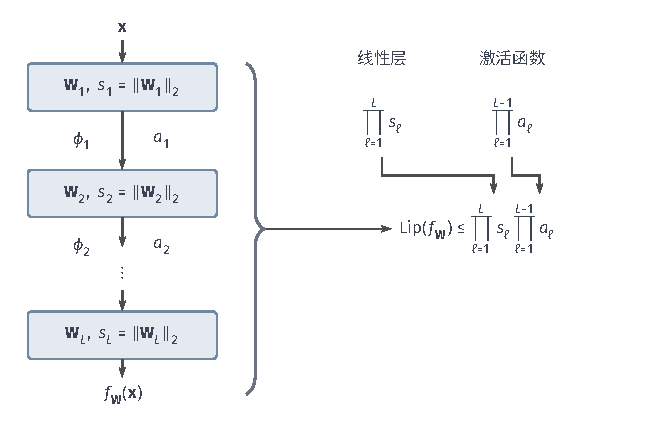
\includegraphics[width=112.000mm]{figures/06-foundations/02-learning-theory/tikz/learning-theory-spectral-product/figure.pdf}
  \caption{谱范数与激活函数共同控制输入扰动。第$\ell$层线性变换至多放大$s_\ell=\|\bm W_\ell\|_2$倍，层间激活再至多放大$a_\ell$倍；末层为线性输出。当激活均为$1$-Lipschitz时，只剩谱范数乘积；该乘积仍不是完整的泛化复杂度。}
  \label{fig:learning-spectral-product}
\end{figure}

放大倍数受控还不等于函数空间简单。谱范数不超过2的矩阵仍有无穷多个，它们指向不同方向，组合出的函数也各不相同。常用的办法是统计覆盖数：在给定精度下，至少需要多少个代表函数，才能使空间中每个函数都离某个代表足够近（可参考\BookVolumeRef{vol:mathematical-preliminaries-upper}{卷1《数学准备：计算、分析与几何》}）。谱范数只记录一层在最强方向上的放大倍数，却看不出这一层“同时用了多少方向”。两个谱范数都为1的矩阵，一个只有一行非零，只能沿一个方向读取输入；另一个是单位矩阵，可以在所有方向上分别读取，后续各层能据此组合出更多不同的函数，覆盖时也需要更多代表。为了把这一差别计入覆盖数，Bartlett等还用到行分组范数，即矩阵各行向量长度之和$\|\bm A\|_{2,1}=\sum_i\|\bm A_{i,:}\|_2$。每一行的长度都不超过谱范数，各行长度之和又不小于谱范数，所以比值$\|\bm A\|_{2,1}/\|\bm A\|_2$总在1与非零行数之间：$100\times100$单位矩阵的比值为100，只有一行非零时为1。这个比值不是秩、稳定秩或奇异方向数：同为秩1，只有一行非零时比值为1，$m$个相同行时比值为$\sqrt m$。对无偏置、$1$-Lipschitz且零点为零的激活网络，Bartlett、Foster与Telgarsky使用的复杂度量（对应文献中取参考矩阵为零的情形）是
\begin{equation}
 \mathcal C(\bm W)=
 \left(\prod_{\ell=1}^L\|\bm W_\ell\|_2\right)
 \left[\sum_{\ell=1}^L
 \left(\frac{\|\bm W_\ell\|_{2,1}}{\|\bm W_\ell\|_2}\right)^{2/3}
 \right]^{3/2}.
 \label{eq:spectral-margin-bound}
\end{equation}
乘积项控制扰动在层间传播时的放大，求和项进入覆盖数的估计；这里按各谱范数非零书写。三层谱范数都为2、比值都为4时，$\mathcal C=8\times(3\times4^{2/3})^{3/2}\approx166$；把每层比值降到1，复杂度降为$8\times3^{3/2}\approx42$。下面采用事先固定范数上限的版本\scite{bartlett2017spectral}。

\begin{theorem}[深层网络的谱复杂度与期望风险]
\label{thm:spectral-network-risk}
设$n,L\geq1$，固定维数$d_0,\ldots,d_L\leq w$且$d_L\geq2$，输入空间
$X\subseteq\mathbb R^{d_0}$取Borel $\sigma$代数，标签空间
$Y=\{1,\ldots,d_L\}$。对
$\bm W_\ell\in\mathbb R^{d_\ell\times d_{\ell-1}}$，定义无偏置网络
\[
\begin{aligned}
 \bm h_0(\bm x)&=\bm x,\\
 \bm h_\ell(\bm x)
 &=\phi_\ell(\bm W_\ell\bm h_{\ell-1}(\bm x)),
 \qquad 1\leq\ell<L,\\
 f_{\bm W}(\bm x)&=\bm W_L\bm h_{L-1}(\bm x),
\end{aligned}
\]
其中各$\phi_\ell$固定、逐坐标作用、为$1$-Lipschitz且在零点为零。间隔按定义~\ref{def:network-margin}，
$\|\bm A\|_{2,1}=\sum_i\|\bm A_{i,:}\|_2$。
设$\mathcal P$为$X\times Y$上的概率分布，
$S=((\bm x_1,y_1),\ldots,(\bm x_n,y_n))\sim\mathcal P^n$，并令
\[
 R^{01}(\bm W)
 =\mathbb P_{(\bm x,y)\sim\mathcal P}
   \{\text{固定平局规则下 }f_{\bm W}\text{ 的预测不等于 }y\}.
\]
在抽样前固定$r,\gamma,s_\ell,b_\ell>0$及$\delta\in(0,1)$，并令
\[
 \mathcal C_0=
 \left(\prod_{\ell=1}^L s_\ell\right)
 \left[\sum_{\ell=1}^L(b_\ell/s_\ell)^{2/3}\right]^{3/2}.
\]
若$\|\bm x\|_2\leq r$在$\mathcal P$下几乎处处成立且$n\geq2$，
则以至少$1-\delta$的概率，
所有满足$\|\bm W_\ell\|_2\leq s_\ell$、
$\|\bm W_\ell\|_{2,1}\leq b_\ell$的网络同时有
\begin{equation}
 R^{01}(\bm W)\leq\hat R_{S,\gamma}(\bm W)+\frac8n
 +\frac{72r\mathcal C_0\log(2w)\log n}{\gamma\sqrt n}
 +3\sqrt{\frac{\log(1/\delta)}{2n}},
 \label{eq:spectral-risk-explicit}
\end{equation}
其中
$\hat R_{S,\gamma}=n^{-1}\sum_i
\mathbb I\{\operatorname{margin}_{\bm W}(\bm x_i,y_i)\leq\gamma\}$
为经验间隔错误率。
\end{theorem}
\begin{proof}
采用Bartlett等论文附录引理A.8的固定范数约束界，其复杂度项为
$72\|\bm X\|_F\mathcal C_0\log(2w)\log n/(\gamma n)$，
其中$\bm X$的各行为训练样本中的输入向量。由$\|\bm x_i\|_2\leq r$得
$\|\bm X\|_F\leq r\sqrt n$，代入即得所述形式。
网络覆盖数的组合估计来自所引外部引理，本章只完成代入这一步。
\end{proof}

上界在经验间隔错误率外保留三项余量；忽略对数因子，使它们不超过$\varepsilon$的门槛为$\bigl((r\mathcal C_0/\gamma)^2+\log(1/\delta)\bigr)/\varepsilon^2$量级。深度和宽度仍通过$\mathcal C_0$及对数参与，因此只替代了粗略的参数计数，没有消除结构的影响。范数乘积、行分组量与间隔共同进入界：复杂度项主导且忽略对数变化时，$\mathcal C_0/\gamma$减半可将同一附加误差的充分样本量约降为四分之一。

这一保证的数值意义需要单独检查。取$r=1$、$\mathcal C_0/\gamma=100$、宽度$w=500$、$n=10^4$，复杂度项约为$72\times100\times\log1000\times\log10^4/100\approx72\times6.9\times9.2\approx4.6\times10^3$，远大于1，此时界不提供任何非平凡的分类保证。这类常数和对数因子使界在常见规模下往往没有数值意义；它更可靠的用途是揭示风险依赖哪些量，以及在其他条件相同时比较不同训练结果。

$\mathcal C$对ReLU网络的等价缩放保持不变。把第一层乘以$c$、第二层除以$c$，网络表示同一函数；谱范数乘积不变，每层的比值$\|\bm W_\ell\|_{2,1}/\|\bm W_\ell\|_2$也不受整体缩放影响。若改用各层谱范数之和，这个和会从$s_1+s_2$变为$cs_1+s_2/c$，对同一函数给出不同复杂度。另一方面，范数上限与间隔尺度在这条定理中必须先于样本固定。若训练后再选择它们，应事先列出一串候选上限（例如$1,2,4,8,\ldots$），对它们同时建立保证，并把失败概率$\delta$分摊到各候选上，代价是多出一个对数项；文献中的自适应版本做的正是这件事。不能把事后测量值直接代入固定约束而遗漏选择代价。

\term{Schatten范数}（Schatten norm）按奇异值的$p$范数（$1\leq p\leq\infty$）汇总矩阵的谱规模；非零矩阵的稳定秩则用总平方谱能量除以最大奇异值平方。这些量与依赖坐标的行分组量不同。不同风险界使用不同谱量，式~\eqref{eq:spectral-margin-bound}采用的是行分组比值，不能直接换成稳定秩。

\subsubsection{矩阵预测的核范数界}

第~\ref{sec:deep-implicit-bias}节得到的是一种动力学偏好：深层分解先学强的谱方向。要把它接到风险，需要一个既能由因子参数控制、又能进入复杂度计算的矩阵量。低秩本身不够，还需要矩阵的总尺度。\term{核范数}（nuclear norm）$\|\bm W\|_*$是奇异值之和，这里的“核”与NTK中的核函数无关；奇异值为$(3,1,0,\ldots,0)$的矩阵，核范数为4。秩至多$q$且$\|\bm W\|_F\leq F$时，Cauchy--Schwarz给出$\|\bm W\|_*\leq\sqrt qF$，所以低秩只有连同受控的尺度，才保证核范数小。因子参数的大小与核范数之间有一个精确的静态关系。

\begin{lemma}[二层分解的范数关系]
\label{lem:factorization-nuclear-norm}
设$\bm W\in\mathbb R^{d_1\times d_2}$，并取
$k\geq\operatorname{rank}(\bm W)$。当
$\bm U\in\mathbb R^{d_1\times k}$、$\bm V\in\mathbb R^{d_2\times k}$时，
\[
 \|\bm W\|_*=\min_{\bm U\bm V^\top=\bm W}
       \tfrac12(\|\bm U\|_F^2+\|\bm V\|_F^2).
\]
\end{lemma}
\begin{proof}
先证下界。核范数与谱范数互为对偶：
\[
 \|\bm W\|_*=\sup_{\|\bm C\|_2\leq1}\langle\bm C,\bm W\rangle_F.
\]
对$\bm W=\bm U\bm V^\top$和任意$\|\bm C\|_2\leq1$，
\[
 \langle\bm C,\bm U\bm V^\top\rangle_F=\sum_k\bm u_k^\top\bm C\bm v_k\leq\sum_k\|\bm u_k\|_2\|\bm v_k\|_2\leq\|\bm U\|_F\|\bm V\|_F,
\]
其中$\bm u_k,\bm v_k$是第$k$列，最后一步用Cauchy--Schwarz；再用$ab\leq(a^2+b^2)/2$得到下界。再证可达。若$\bm W=\bm P\bm\Sigma\bm Q^\top$是紧奇异值分解，取$\bm U=\bm P\bm\Sigma^{1/2}$、$\bm V=\bm Q\bm\Sigma^{1/2}$，两因子的范数平方都等于$\operatorname{tr}\bm\Sigma=\|\bm W\|_*$，从而达到等号。当$k>\operatorname{rank}(\bm W)$时，在两因子后补零列。
\end{proof}

引理联系的是显式因子范数与端到端核范数：在因子上加平方惩罚，等价于在端到端矩阵上加核范数惩罚。它不证明单纯的经验损失梯度流会最小化核范数，第~\ref{sec:deep-implicit-bias}节的谱动力学也不能直接替代这一条件；Razin与Cohen的反例正说明这种替代可能失败。

若训练确实得到受控核范数，再固定它服务的预测问题：输入矩阵$\bm A$，输出$h_{\bm W}(\bm A)=\langle\bm W,\bm A\rangle_F$，内积为对应元素乘积之和。$\bm A$可以选择单个待预测元素（某个位置为1、其余为0），也可以表示多个元素的线性观测。由上面的对偶关系，
\[
 |\langle\bm W,\bm A\rangle_F|\leq\|\bm W\|_*\|\bm A\|_2,
\]
沿$\bm A$最大奇异方向分配全部核范数可取等号。这一关系在模型侧限制总奇异值，在输入侧只用最大方向强度，把矩阵约束接到预测幅度。

\begin{theorem}[基于谱结构的矩阵预测期望风险]
\label{thm:nuclear-norm-generalization}
设$n,d_1,d_2\geq1$，矩阵输入空间为$\mathbb R^{d_1\times d_2}$，
$(Y,\mathcal Y)$为可测标签空间，
$\mathcal P$为$\mathbb R^{d_1\times d_2}\times Y$上的概率分布，且
$S=((\bm A_1,y_1),\ldots,(\bm A_n,y_n))\sim\mathcal P^n$。
假设$\|\bm A\|_F\leq r$在$\mathcal P$下几乎处处成立。
对$\bm W\in\mathbb R^{d_1\times d_2}$，令
$h_{\bm W}(\bm A)=\langle\bm W,\bm A\rangle_F$。
损失$\ell:\mathbb R\times Y\to[0,1]$可测，且关于预测值为$G$-Lipschitz；定义
\[
 R(h_{\bm W})=\mathbb E_{(\bm A,y)\sim\mathcal P}
                    \ell(h_{\bm W}(\bm A),y),\qquad
 \hat R_S(h_{\bm W})=\frac1n\sum_{i=1}^n
                    \ell(h_{\bm W}(\bm A_i),y_i).
\]
固定$B,r,G>0$和$\delta\in(0,1)$，以概率至少$1-\delta$，
所有$\|\bm W\|_*\leq B$同时满足
\[
 R(h_{\bm W})\leq\hat R_S(h_{\bm W})
       +\frac{2GBr}{\sqrt n}
       +3\sqrt{\frac{\log(2/\delta)}{2n}}.
\]
特别地，若对某个矩阵分解训练算法另行证明其输出$\bm W_S$满足
$\|\bm W_S\|_*\leq B$，则$\bm W_S$服从同一个上界。
若进一步规定$q\geq1$、$F>0$、
$\operatorname{rank}(\bm W)\leq q$且$\|\bm W\|_F\leq F$，
可将复杂度项中的$B$取为$\sqrt qF$。
\end{theorem}
\begin{proof}
由核范数与谱范数的对偶关系，对固定的随机符号，
\[
 \sup_{\|\bm W\|_*\leq B}\sum_i\sigma_i\langle\bm W,\bm A_i\rangle_F=B\Bigl\|\sum_i\sigma_i\bm A_i\Bigr\|_2.
\]
于是预测函数类的经验Rademacher复杂度为
\[
 \frac Bn\mathbb E_{\bm\sigma}
       \left\|\sum_{i=1}^n\sigma_i\bm A_i\right\|_2
 \leq\frac Bn\sqrt{\mathbb E_{\bm\sigma}\Bigl\|\sum_{i=1}^n\sigma_i\bm A_i\Bigr\|_F^2}
 =\frac Bn\sqrt{\sum_{i=1}^n\|\bm A_i\|_F^2}
 \leq\frac{Br}{\sqrt n},
\]
其中先用谱范数不超过Frobenius范数与Jensen不等式，再利用随机符号使平方展开的交叉项期望为零。对损失应用引理~\ref{lem:rademacher-contraction}引入因子$G$，再用定理~\ref{thm:rademacher-risk-bound}的经验复杂度形式即得结论。低秩情形由$\|\bm W\|_*\leq\sqrt q\|\bm W\|_F$得到。
\end{proof}

这个证明展示了从矩阵结构到预测保证的实际推导：对偶关系把复杂度变成随机矩阵的谱范数，再用Frobenius范数粗略控制。所列条件下，使附加项至多$\varepsilon$的充分样本量为$O((G^2B^2r^2+\log(1/\delta))/\varepsilon^2)$；秩为$q$且尺度受控时，相应量为$G^2qF^2r^2$。$F,r$仍可能随矩阵规模增长，所以低秩并未无条件消除维度影响。

低秩与受控的总尺度共同给出核范数上界，但深层训练是否达到这些约束仍须另证。风险结论针对的是指定观测分布中的预测：$\bm A$只抽取评分矩阵中某些位置时，低预测风险说明在这类位置上预测准确，不等于完整恢复未知矩阵。未观测方向的信息需要观测位置的覆盖与矩阵结构条件支持：秩为5的$1000\times1000$矩阵约有$10^4$个自由数，与观测数同一量级，但如果观测只集中在前十行，其余行仍可能有多种秩5的补全。

\subsubsection{固定核预测的RKHS范数界}
\label{sec:ntk-rkhs-generalization}

第~\ref{sec:neural-tangent-kernel}节的固定核训练收敛到训练样本上的插值。要估计新输入上的风险，还要用某种“大小”衡量训练得到的函数。线性化模型中最自然的候选是参数位移的欧氏范数$\|\bm v\|_2$，但它衡量的是参数，而风险只取决于函数。若$\bm u$与所有允许输入的梯度特征都正交，则$\bm v$与$\bm v+\bm u$表示同一个线性化函数，参数范数却计入这个不改变函数的分量。所以先对同一函数的全部参数表示取最小范数。

由$K_0$生成的\term{再生核希尔伯特空间}（reproducing kernel Hilbert space, RKHS）记为$\mathcal H_{K_0}$。在当前问题中，可以把它理解为线性化模型能表示的全部函数增量，配上“写出它所需的最短参数位移”这一大小。在$\mathcal H_{K_0}$中，核截面$K_0(\bm x,\cdot)$与函数的内积给出该函数在$\bm x$处的值，即再生性质。在有限维梯度特征下，$g(\bm x)=\langle\bm v,\bm\varphi_0(\bm x)\rangle$的范数为
\[
 \|g\|_{\mathcal H_{K_0}}
 =\inf\{\|\bm v\|_2:g(\bm x)=\langle\bm v,\bm\varphi_0(\bm x)\rangle
                         \text{ 对所有 }\bm x\text{ 成立}\}.
\]
我们控制的是相对于初始化的函数增量$g=f-f_0$，而不是默认$f_0=0$后的整个输出。初始预测非零时，先把它从标签中减去，得到目标残差$r_i=y_i-f_0(\bm x_i)$：训练只需补上剩余部分。

\begin{theorem}[初始梯度特征的最小范数插值]
\label{thm:ntk-minimum-rkhs-norm}
设$X$为非空集合，$K_0:X\times X\to\mathbb R$为正定核，
$\mathcal H_{K_0}$为其RKHS。给定$n\geq1$个输入$\bm x_1,\ldots,\bm x_n\in X$、
实数标签$y_1,\ldots,y_n$和函数$f_0:X\to\mathbb R$，定义
\[
 (\bm K_0)_{i,j}=K_0(\bm x_i,\bm x_j),\qquad
 r_i=y_i-f_0(\bm x_i),\qquad
 \bm r=(r_1,\ldots,r_n)^\top.
\]
假设核矩阵$\bm K_0$正定，并令
$\bm k_0(\bm x)=(K_0(\bm x_i,\bm x))_{i=1}^{n}$。
满足$g(\bm x_i)=r_i$的最小RKHS范数函数为
$\widehat g(\bm x)=\bm k_0(\bm x)^\top\bm K_0^{-1}\bm r$，
其范数满足
\begin{equation}
 \|\widehat g\|_{\mathcal H_{K_0}}^2
 =\bm r^\top\bm K_0^{-1}\bm r
 =\sum_{j=1}^n\frac{(\bm u_j^\top\bm r)^2}{\lambda_j},
 \label{eq:ntk-label-spectral-complexity}
\end{equation}
其中$(\lambda_j,\bm u_j)$为$\bm K_0$的正交特征对。对半平方经验损失
$\mathcal E(g)=\frac1{2n}\sum_i(f_0(\bm x_i)+g(\bm x_i)-y_i)^2$
从$g_0=0$出发的RKHS梯度流
\[
 \dot g_t=-\frac1n\sum_{i=1}^n
 (f_0(\bm x_i)+g_t(\bm x_i)-y_i)K_0(\bm x_i,\cdot)
\]
收敛到$\widehat g$。
\end{theorem}
\begin{proof}
将任意$g$分解为$\operatorname{span}\{K_0(\bm x_i,\cdot)\}_{i=1}^n$中的分量与正交分量。由再生性质，正交分量在各$\bm x_i$处取值为零，去掉它不改变插值条件，也不会增大范数。最小范数函数因而形如$g=\sum_i a_iK_0(\bm x_i,\cdot)$，插值条件为$\bm K_0\bm a=\bm r$，故$\bm a=\bm K_0^{-1}\bm r$，且$\|g\|^2=\bm a^\top\bm K_0\bm a=\bm r^\top\bm K_0^{-1}\bm r$；对核矩阵作谱分解得到第二个等式。梯度流的每个增量都在上述张成空间中，从零出发便始终留在其中；训练点上的预测满足定理~\ref{thm:ntk-training-convergence}的方程，故收敛到插值。张成空间中满足插值条件的函数唯一，所以极限是$\widehat g$。
\end{proof}

式~\eqref{eq:ntk-label-spectral-complexity}按核特征方向计算插值代价：残差在特征值$\lambda_j$方向上的分量越大、$\lambda_j$越小，插值所需的范数就越大。小特征值本身不增加复杂度，只有残差确实需要沿这个方向变化时才付出代价。取
\[
 \bm K_0=\begin{pmatrix}1&1-a\\1-a&1\end{pmatrix},\qquad 0<a\leq1,
\]
其特征值为$2-a$（方向$(1,1)$，两输入同升同降）和$a$（方向$(1,-1)$，一升一降）。残差同为1时全在第一个方向上，范数平方为$2/(2-a)$，不超过2；残差为1和$-1$时全在第二个方向上，范数平方却为$2/a$。取$a=0.01$，后者为200，是前者的约200倍：初始梯度把两个输入判为几乎相同，强制它们取相反输出便需要很大的范数。所以不能仅凭核矩阵正定就判断泛化良好。

要把这一范数接到总体风险，固定独立于样本的核，要求$K_0(\bm x,\bm x)\leq\kappa^2$，即梯度特征范数至多$\kappa$，再事先指定$B$，分析仿射函数类$f_0+\mathcal G_B$，其中$\mathcal G_B=\{g\in\mathcal H_{K_0}:\|g\|_{\mathcal H_{K_0}}\leq B\}$。

\begin{theorem}[初始梯度特征的期望风险界]
\label{thm:ntk-rkhs-risk}
设$(X,\mathcal X)$为可测输入空间，$Y\subseteq\mathbb R$为可测标签空间，
$\mathcal P$为$X\times Y$上的概率分布，且
$S=((\bm x_1,y_1),\ldots,(\bm x_n,y_n))\sim\mathcal P^n$。
函数$f_0:X\to\mathbb R$与可测正定核$K_0:X\times X\to\mathbb R$
在抽样前确定；它们也可随机选取，但须与$S$独立，并且以下条件几乎必然成立。
令$\mathcal H_{K_0}$为$K_0$的RKHS，假设
$K_0(\bm x,\bm x)\leq\kappa^2$对所有$\bm x\in X$成立。
损失$\ell:\mathbb R\times Y\to[0,1]$可测，且关于第一个变量为
$G$-Lipschitz。对任意可测$f:X\to\mathbb R$，定义
\[
 R(f)=\mathbb E_{(\bm x,y)\sim\mathcal P}\ell(f(\bm x),y),\qquad
 \hat R_S(f)=\frac1n\sum_{i=1}^n\ell(f(\bm x_i),y_i).
\]
假设随机变量
$\sup_{g\in\mathcal G_B}|R(f_0+g)-\hat R_S(f_0+g)|$可测。
对任意在抽样前固定的$B,\kappa,G>0$和$\delta\in(0,1)$，以概率至少
$1-\delta$，对所有$g\in\mathcal G_B$同时有
\begin{equation}
 R(f_0+g)\leq\hat R_S(f_0+g)
       +\frac{2G\kappa B}{\sqrt n}
       +3\sqrt{\frac{\log(2/\delta)}{2n}}.
 \label{eq:ntk-rkhs-risk}
\end{equation}
若存在$g_\star\in\mathcal G_B$使
$y=f_0(\bm x)+g_\star(\bm x)$在$\mathcal P$下几乎处处成立，且
$\ell(y,y)=0$，并且样本核矩阵几乎必然正定，则最小范数插值函数
$\widehat g\in\argmin\{\|g\|_{\mathcal H_{K_0}}:f_0(\bm x_i)+g(\bm x_i)=y_i,\ 1\leq i\leq n\}$
满足同一上界且经验风险项为零。对任意$\varepsilon\in(0,1)$，一个充分样本量条件是
\[
 n\geq\max\left\{\frac{16G^2\kappa^2B^2}{\varepsilon^2},
                  \frac{18\log(2/\delta)}{\varepsilon^2}\right\},
\]
此时期望风险以概率至少$1-\delta$不超过$\varepsilon$。
\end{theorem}
\begin{proof}
利用再生性质，$\sup_{\|g\|\leq B}\sum_i\sigma_ig(\bm x_i)=B\|\sum_i\sigma_iK_0(\bm x_i,\cdot)\|_{\mathcal H_{K_0}}$；再由Jensen不等式、再生性质与随机符号交叉项期望为零，
\[
 \widehat{\mathfrak R}_S(\mathcal G_B)
 =\frac Bn\mathbb E_{\bm\sigma}
       \left\|\sum_{i=1}^n\sigma_i K_0(\bm x_i,\cdot)\right\|_{\mathcal H_{K_0}}
 \leq\frac Bn\sqrt{\sum_{i=1}^nK_0(\bm x_i,\bm x_i)}
 \leq\frac{\kappa B}{\sqrt n}.
\]
与所选函数无关的偏移$f_0$不改变复杂度。由收缩性质引入因子$G$，应用定理~\ref{thm:rademacher-risk-bound}的经验复杂度形式，即得式~\eqref{eq:ntk-rkhs-risk}。可实现函数$g_\star$满足所有插值条件，所以最小范数解满足$\|\widehat g\|\leq\|g_\star\|\leq B$，且经验风险为零。分别使风险界两项至多$\varepsilon/2$，得到所列充分样本量。
\end{proof}

复杂度项与第~\ref{sec:rademacher-complexity}节线性分类器的结果形式相同：线性化模型就是以$\bm\varphi_0(\bm x)$为输入、以$\bm v$为系数的线性模型，$\kappa$对应输入长度上限，$B$对应系数范数上限。所以即使特征维数无限，复杂度也由$\kappa B$控制。谱与残差可以共同检验范数条件：只要算出$\sum_j(\bm u_j^\top\bm r)^2/\lambda_j\leq B^2$，就知道插值解落在所控的范数球里。$B$必须事先固定；若观察后才令$B=\|\widehat g\|$，需要对一列预定范数球同时控制，并分摊置信度。

核正定只保证能够插值，不能替代小范数条件。粗略界$\bm r^\top\bm K_0^{-1}\bm r\leq\|\bm r\|_2^2/\lambda_{\min}$中，$\|\bm r\|_2^2$通常随$n$线性增长；若最小特征值只保持常数，$B^2$也随$n$线性增长，代入$\kappa B/\sqrt n$后并不下降。要得到有意义的保证，必须利用残差主要落在大特征值方向这一结构。Arora等对特定两层过参数化网络同时使用标签与核谱，在明确的初始化、宽度和数据条件下得到训练及不显含宽度的样本复杂度保证\scite{arora2019finegrained}。同一个核面对不同的标签方向，可能产生完全不同的风险代价；实际有限网络与固定核模型之间的差异，在第~\ref{sec:network-risk-transfer}节另行控制。

\subsection{算法稳定性界}

复杂度界对整个函数集合同时成立，代价是必须覆盖其中最坏的函数。稳定性只看实际算法：比较只差一个样本的两份训练集分别得到的输出。第~\ref{sec:algorithmic-stability}节已经建立一般结论，定理~\ref{thm:stability-expected-generalization}说，若替换任意一个观测后，任意测试点上的损失至多改变$\beta_n$，则期望泛化差的绝对值至多$\beta_n$。本小节把它用于三种网络描述：分层参数、固定核特征和神经元分布，只展开各自从输出变化到损失变化的新增计算。

\subsubsection{分层参数变化与损失差}

谱复杂度界中的逐层放大计算也可以用于稳定性。现在比较的不再是同一函数空间中的所有网络，而是两份相邻训练集训练出的两个网络。若第$\ell$层参数因替换样本至多改变$\alpha_{\ell,n}$，这一改变会经后续各层继续放大后到达输出。下面的定理因此同时需要两类量：各层范数上限$s_j$控制放大，参数变化$\alpha_{\ell,n}$控制起点处的扰动。

\begin{theorem}[分层参数稳定性与期望泛化差]
\label{thm:layerwise-parameter-stability}
设$n,L\geq1$，$(X,\mathcal X)$为$\mathbb R^{d_0}$的可测子空间，
$(Y,\mathcal Y)$为标签空间，$\mathcal P$为$X\times Y$上的概率分布，且
$S=((\bm x_1,y_1),\ldots,(\bm x_n,y_n))\sim\mathcal P^n$。
固定维数$d_0,\ldots,d_L$，网络按定理~\ref{thm:spectral-network-risk}的形式定义，
各$\phi_\ell$固定、可测、逐坐标作用、为$1$-Lipschitz且在零点为零，
并且$\|\bm x\|_2\leq r$对所有$\bm x\in X$成立。
设可测确定性算法$A$对任意仅有一个观测不同的相邻样本$S,S'$输出
$\bm W=A(S)$、$\bm W'=A(S')$，
且每层均满足$\|\bm W_\ell\|_2,\|\bm W'_\ell\|_2\leq s_\ell$，并有
$\|\bm W_\ell-\bm W'_\ell\|_2\leq\alpha_{\ell,n}$。
设预测损失
$\ell_{\mathrm{pred}}:\mathbb R^{d_L}\times Y\to\mathbb R$可测，并且对所有
$y\in Y$和$\bm u,\bm v\in\mathbb R^{d_L}$都有
$|\ell_{\mathrm{pred}}(\bm u,y)-\ell_{\mathrm{pred}}(\bm v,y)|\leq G\|\bm u-\bm v\|_2$，
其中$r,G,s_\ell,\alpha_{\ell,n}\geq0$，且
$\mathbb E_{y\sim\mathcal P_Y}|\ell_{\mathrm{pred}}(\bm 0,y)|<\infty$。
以$\ell_{\mathrm{pred}}(f_{\bm W}(\bm x),y)$定义$R(\bm W)$与$\hat R_S(\bm W)$，则
\[
 \left|\mathbb E_S\bigl[R(A(S))-\hat R_S(A(S))\bigr]\right|
 \leq Gr\sum_{\ell=1}^L\alpha_{\ell,n}\prod_{j\ne\ell}s_j.
\]
\end{theorem}
\begin{proof}
从$\bm W$出发逐层替换成$\bm W'$：记$\bm W^{[\ell]}$为前$\ell$层取自$\bm W'$、其余层取自$\bm W$的混合参数，则$\bm W^{[0]}=\bm W$、$\bm W^{[L]}=\bm W'$，且
\[
 f_{\bm W}(\bm x)-f_{\bm W'}(\bm x)
 =\sum_{\ell=1}^L\bigl(f_{\bm W^{[\ell-1]}}(\bm x)-f_{\bm W^{[\ell]}}(\bm x)\bigr).
\]
相邻两个混合参数只在第$\ell$层不同。由于激活$1$-Lipschitz且在零点为零，第$\ell$层的输入范数不超过$r\prod_{j<\ell}s_j$；该层输出至多相差$\alpha_{\ell,n}r\prod_{j<\ell}s_j$，再经过后续各层（每层至多放大$s_j$倍，激活不放大），输出差至多为$r\alpha_{\ell,n}\prod_{j\ne\ell}s_j$。把各次替换的输出差相加，再乘损失的Lipschitz常数，便得到损失均匀稳定性上界$\beta_n=Gr\sum_\ell\alpha_{\ell,n}\prod_{j\ne\ell}s_j$。输出范数至多为$r\prod_js_j$，所以零输出处的可积性与Lipschitz条件保证测试损失和训练损失可积。由定理~\ref{thm:stability-expected-generalization}得到结论。
\end{proof}

右侧同时需要$s_j$和$\alpha_{\ell,n}$，二者是不同的条件。只知道范数界时，两次训练的同一层参数最多相差$\alpha_{\ell,n}\leq2s_\ell$，这个量不随$n$变小，上界也就不会消失；必须另外证明算法对单个样本不敏感，例如$\alpha_{\ell,n}$按$1/n$缩小。所以本小节提供的是把已知的参数稳定性转换为网络风险保证的计算，并不声称任意深网的训练都稳定。结论还只针对Lipschitz损失，零一损失须另外借助间隔连接。

\subsubsection{固定特征正则化的稳定性}

固定梯度特征之后，模型$g_{\bm v}(\bm x)=f_0(\bm x)+\langle\bm v,\bm\varphi_0(\bm x)\rangle$对参数$\bm v$是线性的，凸损失下训练目标是凸函数，可以直接使用第~\ref{sec:regularized-learning}节的强凸正则化稳定性。这里需要核对的是网络特征形成的常数。需要注意，“一次训练中核变化很小”说的是同一次训练随时间的变化，并没有说明两份只差一个样本的训练集会得到相近的函数，二者不能互相替代。

\begin{theorem}[正则化固定特征模型的稳定性]
\label{thm:ntk-stability-risk}
设$(X,\mathcal X)$为可测输入空间，$(Y,\mathcal Y)$为可测标签空间，
$\mathcal P$为$X\times Y$上的概率分布，且
$S=((\bm x_1,y_1),\ldots,(\bm x_n,y_n))\sim\mathcal P^n$。
在抽样前固定可测函数$f_0:X\to\mathbb R$和
$\bm\varphi_0:X\to\mathbb R^p$，其中
$\|\bm\varphi_0(\bm x)\|_2\leq\kappa$对所有$\bm x\in X$成立。
设损失$\ell:\mathbb R\times Y\to\mathbb R$可测，关于第一个变量凸且为
$G$-Lipschitz，并满足
$\mathbb E_{(\bm x,y)\sim\mathcal P}|\ell(f_0(\bm x),y)|<\infty$。
以$\ell(g_{\bm v}(\bm x),y)$定义$R(g_{\bm v})$与$\hat R_S(g_{\bm v})$。对$G,\kappa,\lambda>0$，令
\[
 \widehat{\bm v}_S=\argmin_{\bm v\in\mathbb R^p}
 \left\{\hat R_S(g_{\bm v})+\frac\lambda2\|\bm v\|_2^2\right\}.
\]
则算法的均匀稳定性至多为$2G^2\kappa^2/(\lambda n)$，且对任意固定
$\bm v\in\mathbb R^p$，
\[
 \mathbb E_S R(g_{\widehat{\bm v}_S})-R(g_{\bm v})
 \leq\frac{2G^2\kappa^2}{\lambda n}+\frac\lambda2\|\bm v\|_2^2.
\]
\end{theorem}
\begin{proof}
单个样本的损失$\bm v\mapsto\ell(g_{\bm v}(\bm x),y)$是凸函数与仿射映射的复合，因而凸；由Cauchy--Schwarz，它关于$\bm v$为$G\kappa$-Lipschitz。正则项$\frac\lambda2\|\bm v\|_2^2$是$\lambda$-强凸的。定理~\ref{thm:regularized-erm-stability}给出替换一个样本后的参数距离上界$2G\kappa/(\lambda n)$，再乘损失关于参数的Lipschitz常数$G\kappa$，即得均匀稳定性，并由定理~\ref{thm:stability-expected-generalization}控制期望泛化差。正则化最优性还保证
$\hat R_S(g_{\widehat{\bm v}_S})\leq\hat R_S(g_{\widehat{\bm v}_S})+\frac\lambda2\|\widehat{\bm v}_S\|_2^2\leq\hat R_S(g_{\bm v})+\frac\lambda2\|\bm v\|_2^2$。
对样本取期望，并使用固定$\bm v$的经验风险期望等于期望风险，得到结论。
\end{proof}

指定比较半径$B>0$，取$\lambda=2G\kappa/(B\sqrt n)$，两项代价相等，得到
\begin{equation}
 \mathbb E_S R(g_{\widehat{\bm v}_S})
 -\inf_{\|\bm v\|_2\leq B}R(g_{\bm v})
 \leq\frac{2G\kappa B}{\sqrt n}.
 \label{eq:ntk-sample-risk}
\end{equation}
$\lambda$越大，替换一个样本时解的变化越小，但正则化把解拉得离比较参数越远。正则化对核谱的作用可以在平方损失的独立例子中看清。令$r_i=y_i-f_0(\bm x_i)$，目标$\frac1{2n}\sum_i(\langle\bm v,\bm\varphi_0(\bm x_i)\rangle-r_i)^2+\frac\lambda2\|\bm v\|_2^2$的最优参数可写为$\bm v=\sum_i\alpha_i\bm\varphi_0(\bm x_i)$，$\bm\alpha=(\bm K_0+n\lambda\bm I)^{-1}\bm r$。若$\bm K_0\bm u_j=\lambda_j\bm u_j$，残差的第$j$个特征分量在系数中乘以$1/(\lambda_j+n\lambda)$，而不是插值时的$1/\lambda_j$；正则化因此限制了小特征值方向的系数放大。平方损失并非全局Lipschitz，这个谱计算只解释正则化的作用，不能直接套入上面的定理。

这一保证针对指定的固定特征学习问题：特征$\bm\varphi_0$必须在抽样前确定。若特征本身随训练样本改变，例如先训练网络、再冻结所得特征做正则化回归，那么冻结后的特征依赖样本，需要额外控制这种依赖，不能把它当成抽样前固定的特征。它也不直接等于完整非线性网络的训练稳定性。

\subsubsection{神经元分布变化与输出差}

平均场表示把网络写成神经元分布的积分，于是相邻样本的比较可以在分布之间进行。为什么不直接逐个比较两次训练的参数？因为神经元没有固定编号：训练后单元的顺序可能完全打乱，逐个位置比较会把“只是单元顺序不同”的同一网络误判为变化很大。一阶Wasserstein距离先把两个群体中的单元重新配对，再计算配对后参数的平均距离：
\[
 W_1(\mu,\nu)=\inf_{\pi\in\Pi(\mu,\nu)}\mathbb E_{(\bm\vartheta,\bm\vartheta')\sim\pi}\|\bm\vartheta-\bm\vartheta'\|_2,
\]
其中$\Pi(\mu,\nu)$是边缘分别为$\mu$和$\nu$的全部联合分布，每个联合分布就是一种配对方案。一维上把位于0的全部质量搬到1，距离为1；只有一半质量需要从0搬到1，距离为$0.5$。

固定参数域$\Theta\subseteq\mathbb R^q$与输入域，假设单元输出$\psi_{\bm\vartheta}(\bm x)$对参数一致地为$L_\psi$-Lipschitz，即$|\psi_{\bm\vartheta}(\bm x)-\psi_{\bm\vartheta'}(\bm x)|\leq L_\psi\|\bm\vartheta-\bm\vartheta'\|_2$对所有输入成立，预测损失关于输出为$G$-Lipschitz，所涉分布有有限一阶矩。对任意配对$\pi\in\Pi(\rho_S,\rho_{S'})$，由式~\eqref{eq:mean-field-network}，
\[
 |f_{\rho_S}(\bm x)-f_{\rho_{S'}}(\bm x)|
 =\Bigl|\mathbb E_\pi\bigl[\psi_{\bm\vartheta}(\bm x)-\psi_{\bm\vartheta'}(\bm x)\bigr]\Bigr|
 \leq L_\psi\mathbb E_\pi\|\bm\vartheta-\bm\vartheta'\|_2.
\]
等号使用了两个积分分别只依赖各自的边缘分布。对$\pi$取下确界，输出差至多$L_\psi W_1(\rho_S,\rho_{S'})$，任意测试点上的损失差至多$GL_\psi W_1(\rho_S,\rho_{S'})$。若相邻样本训练出的分布总满足$W_1(\rho_S,\rho_{S'})\leq a_n$，由定理~\ref{thm:stability-expected-generalization}，
\[
 \left|\mathbb E_S\bigl[R(f_{\rho_S})-\hat R_S(f_{\rho_S})\bigr]\right|
 \leq GL_\psi a_n.
\]
对$\psi_{(a,\bm w)}(\bm x)=a\phi(\bm w^\top\bm x)$，输入、$a$、$\bm w$有界且激活Lipschitz时，可以验证统一的$L_\psi$存在。再固定允许的分布集合$\mathcal M$，若训练输出$\rho_S\in\mathcal M$且平均经验优化误差至多$\xi_n$，按式~\eqref{eq:deep-risk-decomposition}合并，得到
\begin{equation}
 0\leq
 \mathbb E_S R(f_{\rho_S})
 -\inf_{\rho\in\mathcal M}R(f_\rho)
 \leq G L_\psi a_n+\xi_n.
 \label{eq:mean-field-excess-risk}
\end{equation}
左边非负，Markov不等式可把它转成概率$\mathbb P\{R(f_{\rho_S})-\inf_{\mathcal M}R>\varepsilon\}\leq(GL_\psi a_n+\xi_n)/\varepsilon$；平均界转为高概率界需要付出失败概率的代价。

上面的推导只建立了从“分布稳定”到“泛化差小”的接口。训练算法仍需提供相邻样本对应神经元分布的距离上界$a_n$，这要分析初始化如何耦合、训练多长、损失与势函数的光滑性等；积分表示和距离公式本身不能证明样本稳定性。最终若使用有限宽网络$f_{\rho_{m,S}}$，还须加入它与$\rho_S$之间的近似误差。还需注意，这里的分布组成一个确定的网络函数，与下一小节PAC--Bayes中“从后验抽取完整网络”的随机预测器不是同一对象；后者的分布稳定性在第~\ref{sec:algorithmic-stability}节按完整输出分布另行处理。

\subsection{PAC--Bayes界}
\label{sec:network-pac-bayes}

范数界按参数在最坏方向上的放大倍数计算复杂度，而训练所得的网络往往对许多参数方向上的扰动并不敏感，这一事实在点估计的分析中用不上。PAC--Bayes改为评价训练结果附近的一族网络。第~\ref{sec:pac-bayes}节已经在一般决策空间上建立了这一方法：先验$P$在看到样本前固定，后验$Q$可以依赖样本，从$Q$中抽取一个完整决策再预测，定理~\ref{thm:pac-bayes-bound}以高概率同时控制所有后验的风险。本节直接使用该定理的平方根形式：对$[0,1]$值损失，以至少$1-\delta$的概率，所有$Q\ll P$同时满足
\begin{equation}
 R(Q)\leq\hat R_S(Q)+\sqrt{\frac{D_{\mathrm{KL}}(Q\|P)+\log((n+1)/\delta)}{2n}},
 \label{eq:network-pac-bayes-sqrt}
\end{equation}
其中$\hat R_S(Q)=\mathbb E_{\bm\theta\sim Q}\hat R_S(\bm\theta)$、$R(Q)=\mathbb E_{\bm\theta\sim Q}R(\bm\theta)$。变分不等式、置信转换和互信息分解都不在此重复；本节集中处理网络后验怎样构造、扰动损失和KL代价怎样权衡，以及风险界究竟对应哪个预测器。

\subsubsection{网络先验、后验与经验损失}

对网络，最常见的构造是以训练所得参数$\hat{\bm\theta}$为中心放一个高斯后验$Q=\mathcal N(\hat{\bm\theta},\sigma^2\bm I_p)$，先验取$P=\mathcal N(\bm\theta_P,\tau^2\bm I_p)$。为什么不把后验直接放在$\hat{\bm\theta}$这一个点上？在连续先验下，点质量后验相对先验不绝对连续，KL为无穷，界没有意义；后验必须铺开，把中心附近的完整网络都纳入评价。从$Q$中每抽取一次，就得到一个完整的网络；预测时用的是这个随机网络，这与平均场中“对单元积分得到一个确定网络”不同。

先验与后验对样本的依赖要求不同。后验可以任意依赖训练数据，这是方法允许的部分；先验必须与用于认证的样本独立。先验均值$\bm\theta_P$可以取初始化参数，因为初始化在抽样前完成；若想用部分数据训练出更好的先验，就要把数据划分开，先验只用一部分，界只在其余样本上计算，或使用允许数据依赖先验的相应定理。

代入式~\eqref{eq:network-pac-bayes-sqrt}需要两个量。后验经验损失$\hat R_S(Q)$是随机网络在训练集上的平均损失，一般没有闭式，需要从$Q$抽取若干网络用蒙特卡洛估计，估计误差另需一个置信项；KL代价则对高斯分布有闭式。

\subsubsection{扰动损失、平坦性与复杂度}

对$p$维各向同性高斯，两个分布的相对熵为
\begin{equation}
 D_{\mathrm{KL}}(Q\|P)=\frac{\|\hat{\bm\theta}-\bm\theta_P\|_2^2}{2\tau^2}
 +\frac p2\left(\frac{\sigma^2}{\tau^2}-1-\log\frac{\sigma^2}{\tau^2}\right).
 \label{eq:gaussian-pac-bayes-kl}
\end{equation}
它由各坐标独立的一维高斯相对熵$\frac{(\mu_Q-\mu_P)^2}{2\tau^2}+\frac12\bigl(\frac{\sigma^2}{\tau^2}-1-\log\frac{\sigma^2}{\tau^2}\bigr)$对$p$个坐标求和得到。第一项是中心离先验均值多远，第二项是后验宽度与先验宽度不一致的代价，它在$\sigma^2=\tau^2$处为零，向两侧偏离都增大，并且乘着参数维数$p$。例如$p=10^6$、$\sigma^2=\tau^2/2$时，第二项为$\tfrac{10^6}2(\tfrac12-1+\log2)\approx9.7\times10^4$；若样本数只有$10^5$，式~\eqref{eq:network-pac-bayes-sqrt}中的根号项就接近$0.7$，几乎没有信息。

于是出现一个取舍。扩大后验方差$\sigma^2$，使之接近$\tau^2$，能减轻宽度不一致的代价；但扰动越大，随机网络偏离中心越远，扰动后的训练损失$\hat R_S(Q)$可能上升。只有当损失在中心附近的大范围内都保持很低时，后验才能铺得宽而不付出经验损失。这正是“平坦”最小值被认为有助于泛化的理由；用层间扰动或局部二阶近似估计损失变化时，须明确扰动的局部范围、损失有界性和近似误差。

但平坦性必须落实为“扰动后损失增加多少”与“相对熵代价”的比较，不能单看坐标中的谷宽。图~\ref{fig:learning-flat-sharp}固定一个参数方向，比较同等扰动下两种谷的经验风险增幅。宽谷在此方向上增幅较小，说明局部扰动代价较低；但如图~\ref{fig:lt8-relu-rescaling}所示，把相邻两层分别乘以$c$和$1/c$不改变函数，却能把一个方向上的谷压窄、另一个方向上的谷拉宽，Hessian的特征值随之改变\scite{dinh2017sharp}。所以原始坐标中的平坦性不是独立于参数表示的泛化证据；评价扰动必须与先验的尺度一致。Hessian较小、一次随机扰动没有降低准确率，或中心网络训练损失低，都不能独自替代风险保证。

\begin{figure*}[htbp]
  \centering
  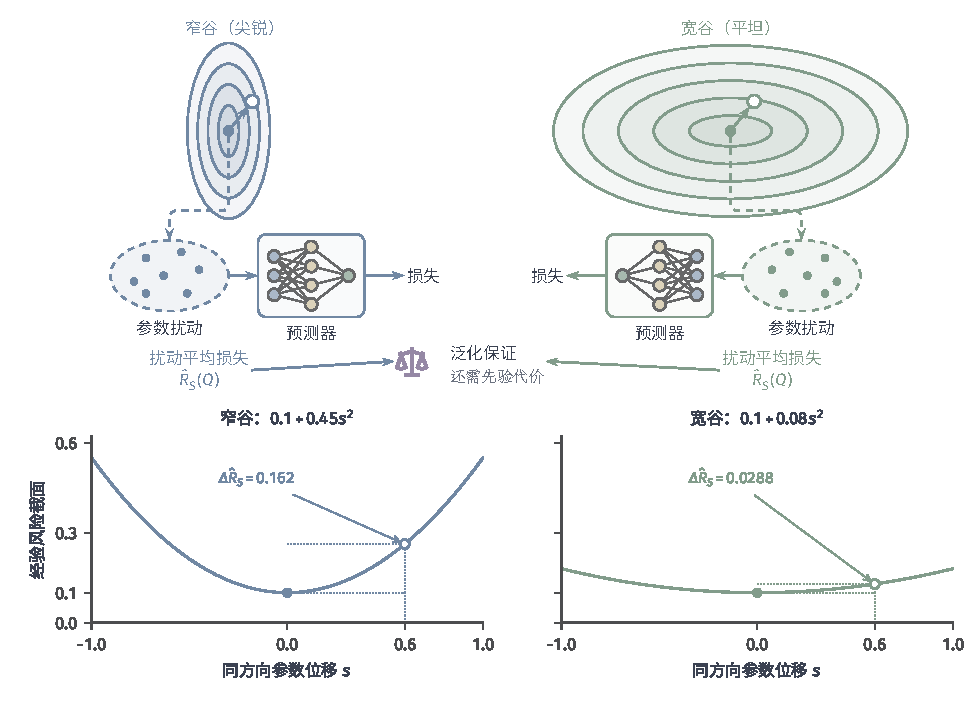
\includegraphics[width=164.600mm]{figures/06-foundations/02-learning-theory/tikz/learning-theory-flat-sharp/figure.pdf}
  \caption{参数扰动代价与PAC--Bayes中的两项控制。上部示意窄谷、宽谷附近的参数扰动与随机预测器；泛化保证还需同时控制后验经验风险与相对于独立先验的相对熵代价。下部两个面板共用相同尺度，横轴为同一单位方向上的参数位移$s$，即$\bm\theta=\hat{\bm\theta}+s\bm u$、$\|\bm u\|_2=1$。构造的窄谷与宽谷分别为$0.1+0.45s^2$、$0.1+0.08s^2$；空心点对应相同位移$s=0.6$，经验风险分别增加$0.162$和$0.0288$。上部轮廓没有数值含义，下部曲线仅为可复算的教学构造。谷的宽度受参数化与坐标尺度影响，宽谷不必具有较小的期望风险。}
  \label{fig:learning-flat-sharp}
\end{figure*}

\subsubsection{风险界对应的预测器}

PAC--Bayes界直接评价的是随机预测器：每次预测前从$Q$抽取一个网络。它与另外两个对象不同：后验平均预测$\bm x\mapsto\mathbb E_{\bm\theta\sim Q}f_{\bm\theta}(\bm x)$，以及固定的中心网络$f_{\hat{\bm\theta}}$。定理~\ref{thm:pac-bayes-bound}首先适用于它声明的随机预测器；转向中心网络或投票分类器时需要额外的关系，例如损失的Lipschitz性、间隔或凸性，不能在解释实验时悄悄更换风险对象。

固定特征模型提供了一个可以完整计算的桥接。设初始函数$f_0$与特征映射$\bm\varphi_0:X\to\mathbb R^p$在抽样前确定，$\|\bm\varphi_0(\bm x)\|_2\leq\kappa$，记$g_{\bm v}=f_0+\langle\bm v,\bm\varphi_0\rangle$。损失取值于$[0,1]$，且对全部扰动后的得分关于得分是全局$G$-Lipschitz的。事先选定$s>0$，取先验$P=\mathcal N(0,s^2\bm I_p)$；训练得到位移$\widehat{\bm v}$后取后验$Q=\mathcal N(\widehat{\bm v},s^2\bm I_p)$。两者协方差相同，式~\eqref{eq:gaussian-pac-bayes-kl}的第二项为零，$D_{\mathrm{KL}}(Q\|P)=\|\widehat{\bm v}\|_2^2/(2s^2)$。

接着把随机预测转回中心。对$\bm v\sim Q$，扰动得分$\langle\bm v-\widehat{\bm v},\bm\varphi_0(\bm x)\rangle$服从均值为零、方差为$s^2\|\bm\varphi_0(\bm x)\|_2^2$的正态分布，其绝对值期望至多$s\kappa$。由Lipschitz性，任意观测上随机预测的期望损失与中心预测的损失相差至多$Gs\kappa$。这一转换在经验风险和总体风险上各用一次：$\hat R_S(Q)\leq\hat R_S(g_{\widehat{\bm v}})+Gs\kappa$，$R(g_{\widehat{\bm v}})\leq R(Q)+Gs\kappa$。代入式~\eqref{eq:network-pac-bayes-sqrt}，以概率至少$1-\delta$，所有中心同时有
\begin{equation}
 R(g_{\widehat{\bm v}})\leq\hat R_S(g_{\widehat{\bm v}})+2Gs\kappa
 +\sqrt{\frac{\|\widehat{\bm v}\|_2^2/(2s^2)+\log((n+1)/\delta)}{2n}}.
 \label{eq:ntk-pac-bayes-risk}
\end{equation}
若$\widehat{\bm v}$取线性化插值的最小范数表示，则$\|\widehat{\bm v}\|_2^2=\|\widehat g\|_{\mathcal H_{K_0}}^2=\bm r^\top\bm K_0^{-1}\bm r$，与式~\eqref{eq:ntk-label-spectral-complexity}的核谱量相同。两条分析路线由此评价同一个训练结果：Rademacher路线在预定的范数球上取上确界，PAC--Bayes路线把同一个范数写成信息代价。

这个构造有几项不能省略的条件。扰动尺度$s$必须事先选定，因为先验依赖它；$s$增大使KL代价减小，却使扰动代价$2Gs\kappa$增大，若插值范数统一有界，预先取$s=n^{-1/4}$可使两项都随$n$下降，但速率比Rademacher界慢。各向同性高斯只在有限维参数空间中直接可用；无限维RKHS中不存在协方差为$s^2I$的高斯概率分布，那里仍应使用前面的复杂度证明。判断一项PAC--Bayes保证是否有数值意义，要同时检查随机化训练损失的估计误差、KL代价、置信水平，以及最终上界是否小于平凡的上界1。若只能说明依赖关系，或所得界仍然宽松，应据实表述，不把公式中的相对改善当成已认证的测试性能。

\subsection{有限网络的风险转移}
\label{sec:network-risk-transfer}

前面的固定核界与平均场界都针对近似模型。实际部署的是有限宽网络$f_S$，与之对应的近似模型输出记为$g_S$，例如线性化模型训练所得的函数。训练点上的逼近不足以把$g_S$的风险传给$f_S$：第~\ref{sec:deep-training-dynamics}节的数值例子已经显示，训练点上核漂移小，也可能在小特征值方向上留下可观的差别，而风险由新输入决定。

所需的条件是在测试分布下控制两者的输出差。若以概率至少$1-\delta_{\mathrm{app}}$（对样本、初始化及算法随机性）满足
\[
 \mathbb E_{\bm x\sim\mathcal P_X}|f_S(\bm x)-g_S(\bm x)|\leq\tau_n,
\]
则对关于预测值$G$-Lipschitz的损失，$|R(f_S)-R(g_S)|\leq\mathbb E_{(\bm x,y)}|\ell(f_S(\bm x),y)-\ell(g_S(\bm x),y)|\leq G\tau_n$。对$\mathcal P_X$几乎处处一致的$\tau_n$界同样足够。近似成立的事件需与复杂度事件一起计入失败概率，例如与定理~\ref{thm:ntk-rkhs-risk}合并时总失败概率至多$\delta+\delta_{\mathrm{app}}$；近似定理通常只在给定的训练时间区间内成立，所用的训练时间也必须落在其中。

完整的保证于是并列三部分：近似模型自身的风险保证，来自复杂度或稳定性分析；有限网络与近似模型的输出差$G\tau_n$，来自网络训练的近似定理；以及训练拟合的程度，来自优化分析。有限网络产生显著特征变化时，$\tau_n$不再小，应重新选择适用的分析和所需条件，例如转向平均场描述，而不是继续使用未经验证的固定核保证。

\section{训练现象}
\label{sec:training-phenomena}

前三节分别回答了训练得到什么、什么条件能保证它的风险。本节反过来，从三个在实验中反复出现的现象出发，检验这些分析能解释到哪一步。三个现象观察的对象不同：双重下降观察的是测试风险怎样随模型规模或训练时间变化；延迟泛化观察的是训练拟合与测试改善在时间上的分离；神经坍缩观察的是训练后期最后一层表示的几何形状。每个案例都按同一顺序展开：先说清楚看到了什么、在什么设定下看到，再介绍已有的机制证据，最后指出这些证据能推出什么、不能推出什么。三个现象有时同时出现，但本节不预设它们有共同的原因。

\subsection{双重下降}
\label{sec:double-descent}

\subsubsection{模型规模与训练时间上的双重下降}

经典的偏差与复杂度权衡（第~\ref{chap:statistical-learning-framework}章）给出一条U形曲线：模型太简单时近似误差大，太复杂时估计误差大，中间某处测试风险最低。可是在许多现代实验中，把模型继续加大到能把训练数据完全插值之后，测试风险先在插值附近急剧上升，随后又重新下降，有时还降到比U形曲线谷底更低。这种“下降—上升—再下降”的曲线称为\term{双重下降}（double descent）。Belkin等人在随机特征、神经网络和决策树等模型上系统描述了这一形状，并把插值点附近的上升与插值解的病态联系起来\scite{belkin2019double}。

先看一个能完整计算的例子。图~\ref{fig:lt8-random-feature-double-descent}来自本书运行的合成实验：输入$\bm x\in\mathbb R^{20}$，真实标签$y=\bm\beta^\top\bm x+\xi$，噪声标准差为0.5，即噪声方差为0.25；训练样本$n=100$。模型取$N$个随机ReLU特征$\phi_j(\bm x)=\max\{\bm v_j^\top\bm x,0\}$，$\bm v_j$在抽样前随机固定，只学习输出层系数。$N<n$时用普通最小二乘，$N\geq n$时方程组有无穷多个插值解，取其中欧氏范数最小者，这正是第~\ref{sec:linear-implicit-bias}节中零初始化梯度下降会选到的解。

\begin{figure}[htbp]
  \centering
  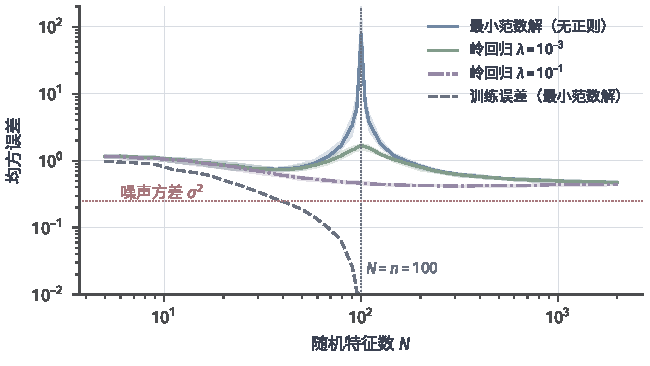
\includegraphics[width=112mm]{figures/06-foundations/02-learning-theory/matplotlib/lt8-random-feature-double-descent/figure.pdf}
  \caption{随机特征回归中测试误差随特征数$N$的变化（本书合成实验）。输入维数20，训练样本$n=100$，噪声方差0.25；实线为40次独立重复的中位数，阴影为四分位区间。最小范数解在$N=n$处测试误差达到约76，两侧都远低于此；岭回归正则化越强，峰越低，$\lambda=10^{-1}$时峰完全消失。虚线为最小范数解的训练误差，$N\geq n$时为零。}
  \label{fig:lt8-random-feature-double-descent}
\end{figure}

读这张图要同时看三条曲线。训练误差（虚线）随$N$单调下降，在$N=n$时变为零并保持为零。最小范数解的测试误差先从约1.16降到$N=37$时的约0.74，然后上升，在$N=n=100$时中位数达到约76，比任何其他位置高出两个数量级；越过这一点后又一路下降，到$N=2000$时约为0.47，低于$N<n$区域的最好水平。岭回归加入$\lambda\|\bm c\|_2^2$以后，$\lambda=10^{-3}$时峰降到约1.7，$\lambda=10^{-1}$时峰完全消失，曲线几乎单调下降。

峰出现在$N=n$并不偶然。$N$略小于$n$时，最小二乘解要用恰好够用的参数去拟合带噪声的标签；$N=n$时，特征矩阵$\bm\Phi\in\mathbb R^{n\times N}$是方阵，插值解为$\bm c=\bm\Phi^{-1}\bm y$。随机方阵的最小奇异值往往很小，它在噪声方向上的放大倍数是$1/\sigma_{\min}(\bm\Phi)$，于是噪声$\bm\xi$被成倍放大进系数，新输入上的预测随之剧烈波动。$N$远大于$n$时，满足插值的解构成一个高维仿射子空间，最小范数解可以在其中挑一个系数较小的，$\bm\Phi$的非零奇异值也远离零，噪声的放大被削弱。岭回归直接把$1/\sigma$换成$\sigma/(\sigma^2+\lambda)$，在小奇异值方向上截断放大，所以峰被压平。这一解释对应第~\ref{sec:benign-overfitting}节的线性分析：插值后风险是否小，取决于特征协方差的谱与噪声，而不是参数个数本身。

Nakkiran等人在卷积网络、残差网络和Transformer上观察到同样的形状，并把它推广到两个新的横轴\scite{nakkiran2020deepdd}。其一是固定架构、改变训练轮数：测试误差随训练时间也可能先降、再升、再降，称为按训练时间的双重下降。其二是固定模型、改变样本量：在插值阈值附近，增加训练样本可能反而使测试误差变大。他们报告，标签噪声越大，峰越明显；数据增强或适当正则化会削弱峰。他们还提出“有效模型复杂度”的假说：把模型规模、训练时长等因素合并成训练程序能在一定训练误差内拟合的最大样本量，峰出现在这一量接近训练样本量的位置。原文明确把它作为统一各种横轴的经验假说，而非证明了的定理。

由此可以得到三点限制。第一，横轴必须写明：按模型规模、按训练时间和按样本量的曲线来自不同实验，不能拼成同一条规律。第二，峰的高度依赖噪声、正则化与训练是否完成；图~\ref{fig:lt8-random-feature-double-descent}中的强岭回归就没有峰。第三，双重下降描述的是一条曲线的形状，不等于“参数越多越好”或“训练越久越好”：在峰的右侧继续加大模型确实降低了这里的测试误差，但这依赖于这个设定中的谱结构与噪声水平。

\subsubsection{网络插值与良性过拟合的条件}

双重下降的右半段提出一个问题：插值了带噪声的训练标签，为什么测试风险还能很低？第~\ref{sec:benign-overfitting}节在线性回归中回答过这个问题：当输入协方差的谱有足够多的“小方向”可以吸收噪声，而少数“大方向”承载信号时，最小范数插值的超额风险可以趋于零，这称为良性过拟合；若谱衰减得太快或太慢，同样的插值是有害的。决定性的是协方差的有效秩，而不是参数个数超过样本数这件事本身\scite{bartlett2020benign}。

把这一结论用到网络上要分两种情况。若训练处在第~\ref{sec:neural-tangent-kernel}节的固定核区域，网络近似为初始梯度特征上的线性模型，就可以检查核矩阵的谱与噪声模型是否满足线性理论的条件；第~\ref{sec:ntk-rkhs-generalization}节的RKHS范数界也给出了插值解的风险上界。若特征在训练中显著移动，特征本身依赖训练样本，训练后测得的谱不再是抽样前固定的，就不能把它直接代入固定特征的定理。

还要把两个概念分开。良性过拟合是一个关于风险的性质：在明确的损失、噪声模型和比较基准下，插值解的超额风险很小。双重下降是一个关于曲线的观察：风险随某个变量先升后降。二者可以同时出现，例如图~\ref{fig:lt8-random-feature-double-descent}右半段的最小范数插值；但出现峰不说明右侧一定良性，没有峰的岭回归也不需要插值。线性理论为网络提供了受控的参照，网络特有的特征形成与优化条件仍要另行证明。

\subsection{延迟泛化：Grokking}
\label{sec:grokking}

\subsubsection{现象与原始实验设定}

Power等人在一类小型算法任务上观察到一个反直觉的训练过程\scite{power2022grokking}。任务是学习一张有限的运算表，例如模$p$加法$c=(a+b)\bmod p$：全部$p^2$个输入对中取一部分作训练，其余作检验，检验的是同一条运算规则能否被推广到没见过的输入对。训练准确率很快接近100\%，检验准确率却长时间停在随机水平附近，要再训练多一到两个数量级的步数，才突然升到接近100\%。这种训练拟合与泛化在时间上的分离称为\term{延迟泛化}，原文称为grokking。他们还报告，训练集比例越小，延迟越长；权重衰减能显著缩短延迟。

图~\ref{fig:lt8-grokking-fourier}的左图是本书按相同思路运行的小实验，设定比原文更简单：$p=47$，随机取40\%的输入对训练，网络先把$a$、$b$各查一个32维嵌入，拼接后经过128个ReLU单元，再输出47个类别分数；用AdamW全批量训练两万步，比较三种解耦权重衰减系数。三次运行的训练准确率都在约100步内达到99\%。权重衰减为1时，检验准确率在约5200步才过半、约6700步达到99\%；系数为0.3时延迟更长，到两万步才达到99\%以上；没有权重衰减时，两万步内检验准确率始终停在随机水平之下。

\begin{figure*}[htbp]
  \centering
  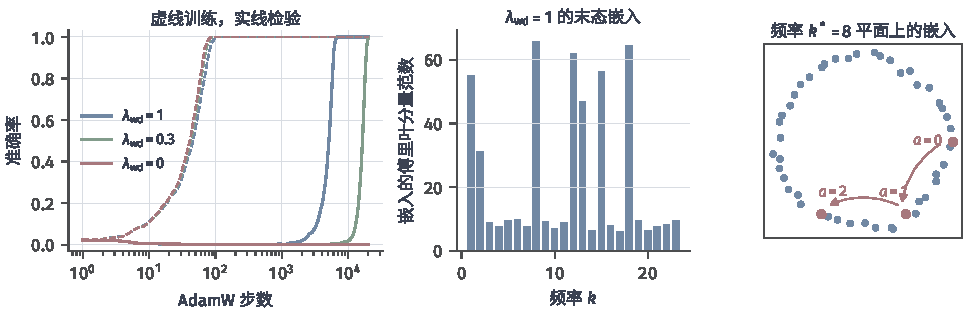
\includegraphics[width=165mm]{figures/06-foundations/02-learning-theory/matplotlib/lt8-grokking-fourier/figure.pdf}
  \caption{模47加法上的延迟泛化与嵌入的傅里叶结构（本书合成实验，不是原论文设定）。左：三种解耦权重衰减系数下的训练准确率（虚线）与检验准确率（实线），横轴为对数刻度的AdamW步数。中：权重衰减为1时末态嵌入沿输入维作离散傅里叶变换后各频率分量的范数，少数频率占主导，前五个频率约占总能量的81\%。右：各输入$a$的嵌入投影到最强频率$k^\star=8$所对应的二维平面上，点按$a$排成一个圆，相邻的$a$相差固定角度$2\pi k^\star/47$。}
  \label{fig:lt8-grokking-fourier}
\end{figure*}

阅读这类曲线时要同时报告网络、优化器、训练比例、权重衰减和训练长度，它们共同构成实验条件；任何一项改变，延迟都可能变长、变短或消失。还要区分两件事：检验准确率迟迟没有提高，不等于网络内部没有形成任何可推广的结构。下一小节的案例正是通过检查内部表示，看到了准确率曲线上看不到的进展。延迟泛化也不要求出现双重下降的完整曲线。

\subsubsection{模运算中的电路形成与清理}

Nanda等人选择单层Transformer的模加法作为可以完整追踪的案例\scite{nanda2023progress}。他们发现，训练后的网络实际执行的是一个基于离散傅里叶变换的算法：把输入$a$、$b$映射到少数几个频率$k$上的$\cos(2\pi ka/p)$、$\sin(2\pi ka/p)$，借三角恒等式
\[
 \cos\frac{2\pi k(a+b)}p=\cos\frac{2\pi ka}p\cos\frac{2\pi kb}p-\sin\frac{2\pi ka}p\sin\frac{2\pi kb}p
\]
在隐藏层中算出$a+b$对应的旋转角，再对每个候选$c$计算$\cos(2\pi k(a+b-c)/p)$，它在$c=a+b\bmod p$时取最大值1。证据来自三方面：嵌入与权重在傅里叶基下集中在少数频率上；激活呈现相应的周期结构；把关键频率的分量消去会显著提高损失，只保留这些分量则几乎不影响损失。

这个算法为什么能推广？因为它对所有$p^2$个输入对用同一套旋转与比较，一旦在训练对上学成，检验对上也同样成立；而逐对记住答案的查表方法对检验对毫无帮助。图~\ref{fig:lt8-grokking-fourier}的中图和右图在本书的小网络中也看到了类似的结构：权重衰减为1的末态嵌入集中在少数频率上，投影到最强频率$k^\star=8$的平面后，47个嵌入排成一个圆，$a$每增加1，点沿圆转过同一个角度，这正是旋转表示的样子。不过本书的网络是MLP而非Transformer，这里只说明嵌入呈现傅里叶结构，没有像原文那样逐层验证完整电路。

Nanda等人用这些量作为“进展度量”，把训练分成三个阶段：先是记忆训练数据；接着，在检验准确率仍然很低时，傅里叶电路就已逐渐形成；最后，权重衰减把起记忆作用的成分清理掉，检验准确率随之跃升。按这个描述，突然的泛化不是突然学会，而是此前已经形成的泛化电路在清理之后终于主导了输出。这一阶段描述依赖模加法的特定结构和消融证据，不能单凭两条准确率曲线推出，也不能预设所有延迟泛化都是在学习傅里叶特征。

\subsubsection{不同解释与实验边界}

电路分析追踪的是一个具体模型内部的计算。另一条研究路线关注训练路径与参数尺度。Liu、Michaud与Tegmark提出，在许多任务中，训练损失与检验损失作为参数范数的函数呈现不同形状：训练损失在较大范数范围内都很低，检验损失只在某个中等范数区间内低\scite{liu2023omnigrok}。若初始化范数远大于这一区间，网络先在大范数处拟合训练数据，权重衰减再慢慢把范数拉回能泛化的区间，于是出现延迟。按这个思路，他们把初始化放大，在MNIST图像分类、IMDb情感分类等非算法任务上也诱发了延迟泛化。Kumar等人则在受控的两层网络模型中把这一过程刻画为从惰性训练到特征学习的转变：网络先像第~\ref{sec:neural-tangent-kernel}节的固定核模型那样拟合训练数据，之后特征才开始移动，泛化随之出现；转变何时发生，取决于特征学习的速率以及初始特征与目标任务的对齐程度\scite{kumar2024grokking}。

这些解释与电路案例并不矛盾，但研究的对象不同：前者研究训练路径和尺度，后者追踪具体的计算结构。把它们合并成“权重衰减必然把记忆变成规则”这样的统一定律，超出了任何一项证据的范围。图~\ref{fig:lt8-grokking-fourier}中不加权重衰减就不发生泛化，与尺度路线的预测一致；但这只是一个小实验在一种设定下的观察。

实现细节也可能改变观察。Prieto等人发现，在模运算等设定中，训练后期logit不断增大，softmax的浮点计算出现吸收误差：正确类的概率在有限精度下被舍入为1，相应的梯度变为零，学习因此停滞\scite{prieto2025grokking}。他们称之为softmax坍缩，并表明改用数值更稳定的softmax替代形式或调整梯度方向，可以在不加权重衰减时也得到泛化。所以“是否出现延迟泛化”不能只归因于范数或权重衰减，数值精度与损失的计算形式也是实验条件的一部分。

综合起来，解释或复现延迟泛化时应报告：任务及其规模、训练集比例、网络与优化器、初始化尺度、正则化方式与强度、训练长度，以及数值精度和损失实现。已有结论分三类：受控模型中证明或精确刻画的机制（如固定核到特征学习的转变），具体案例中有消融证据支持的阶段描述（如模加法电路），以及跨任务的经验规律与研究假说（如范数区间的解释）。延迟泛化至今没有适用于任意网络的统一解释。

\subsection{神经坍缩}
\label{sec:neural-collapse}

\subsubsection{神经坍缩的四种几何关系}

训练一个$K$类分类网络时，训练分类误差通常很早就接近零，而交叉熵损失还会继续下降很久。Papyan、Han与Donoho在这一“终末阶段”测量了最后一层的几何结构，在多个标准图像数据集和架构上观察到四种同时出现的趋势，合称\term{神经坍缩}（neural collapse）\scite{papyan2020neuralcollapse}。记第$k$类训练样本的最后一层特征为$\bm h_{k,i}$，类均值为$\bm\mu_k$，全体均值为$\bm\mu_G$，分类器第$k$行为$\bm w_k$。四种趋势是：
\begin{enumerate}
 \item 类内坍缩：同类样本的特征向类均值聚拢，类内协方差相对类间协方差趋于零；
 \item 类均值趋向等角紧框架：中心化类均值$\bm\mu_k-\bm\mu_G$长度趋于相等，两两夹角的余弦趋于$-1/(K-1)$，也就是正则单纯形的顶点方向；
 \item 自对偶：分类器的行$\bm w_k$与对应的中心化类均值方向趋于一致；
 \item 决策简化：网络的分类结果趋于与“分到最近的类均值”的规则一致。
\end{enumerate}
第二条中的$-1/(K-1)$是$K$个等长、两两等角且和为零的向量所能达到的唯一夹角：若$\sum_k\bm u_k=\bm 0$且$\|\bm u_k\|=1$，则$0=\|\sum_k\bm u_k\|^2=K+K(K-1)c$，解得$c=-1/(K-1)$。$K=3$时为$-1/2$，三个方向互成$120^\circ$。

比较这些关系时要用中心化与归一化后的量，例如类内与类间散度之比、中心化类均值长度的变异系数、分类器方向与类均值方向的余弦。标准表述需要特征维数至少为$K-1$、各类样本数大致平衡。原研究提供的是若干架构与数据集上的系统观察，量的变化是“趋向”某种结构；不能写成任意网络在有限训练时间内必然精确达到。

\subsubsection{无约束特征模型的解释}

为了理解这种几何为什么会出现，可以删去从输入到特征的网络约束：把每个训练样本的最后一层特征$\bm h_i$本身当作自由变量，与分类器$\bm W$一起最小化
\[
 \frac1N\sum_{i=1}^N\ell_{\mathrm{CE}}(\bm W\bm h_i,y_i)
 +\frac{\lambda_W}2\|\bm W\|_F^2+\frac{\lambda_H}2\|\bm H\|_F^2,
\]
其中$\bm H$是全部特征按列排成的矩阵。这称为\term{无约束特征模型}。它的直觉是：深网络表达力足够强时，可以把训练样本的特征放到几乎任意位置，于是特征的排布主要由最后一层的目标决定。Zhu等人证明，在类别平衡、特征维数不小于$K-1$以及他们规定的正则化条件下，这个目标的全局最优解恰好满足神经坍缩的四条关系；而且目标没有虚假的局部最小值，每个其他临界点都是严格鞍点，因而梯度类方法在一般条件下不会被困住\scite{zhu2021ncgeometric}。

图~\ref{fig:lt8-neural-collapse}在最小的非平凡情形里演示这一结论：$K=3$类、每类10个样本，特征维数$d=2=K-1$，特征与分类器都从小随机值开始，用全批量梯度下降最小化上式，取$\lambda_W=\lambda_H=5\times10^{-3}$。初始时三类特征混杂，类内与类间散度之比约为14；第100步时各类已大致分开，但类内仍有散布，类均值长度也不相等；到两万步时，每类的10个特征重合到一点，三个中心化类均值等长、两两余弦为$-1/2$，分类器的三行与对应类均值方向完全对齐。右图的三条度量都下降到数值零附近。

\begin{figure*}[htbp]
  \centering
  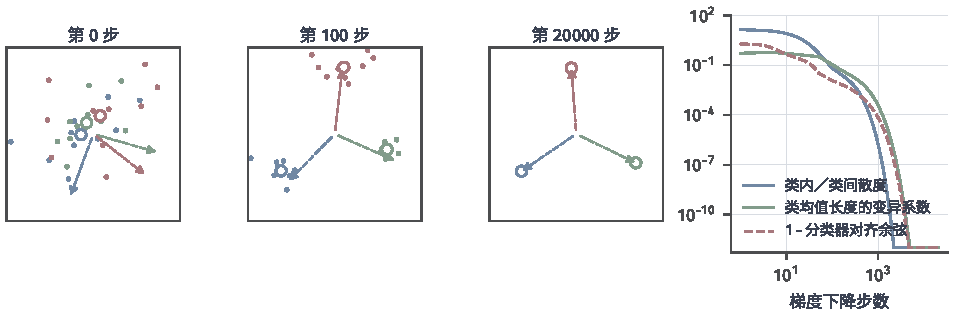
\includegraphics[width=165mm]{figures/06-foundations/02-learning-theory/matplotlib/lt8-neural-collapse/figure.pdf}
  \caption{无约束特征模型中的神经坍缩（本书合成实验）。三类、每类10个样本、二维特征，交叉熵加二次正则（$\lambda_W=\lambda_H=5\times10^{-3}$），全批量梯度下降。左三图为第0、100、20000步的特征（小点）、中心化类均值（空心圆）与分类器各行的方向（虚线箭头），颜色表示类别；末态三个类均值两两成$120^\circ$，分类器方向与之重合。右图为类内与类间散度之比、中心化类均值长度的变异系数和$1-$分类器对齐余弦随步数的变化，低于$10^{-12}$的值贴在下限。}
  \label{fig:lt8-neural-collapse}
\end{figure*}

这个模型为什么偏爱等角结构？可以按目标的两部分分开看。交叉熵要求每个样本的正确类分数比其余类大得越多越好，而两项二次正则限制特征和分类器的总规模；在总规模给定时，把一个类内部的特征散开只会让其中一部分样本的间隔变小，所以最优解把同类特征压到一点，这是类内坍缩。各类之间，交叉熵惩罚的是与最近竞争类的分数差，类别平衡时目标对类的置换对称，最优的排布是让每两类都“同样远”，在和为零的约束下这只能是等角紧框架。分类器与特征共同出现在双线性项$\bm w_k^\top\bm h_i$中，又被同样形式的二次项约束，最优时两者方向一致，这是自对偶；自对偶加上类内坍缩，最大分数规则就等价于最近类均值规则。以上是对最优解结构的直观解释，严格结论及其条件以Zhu等人的定理为准。

还要把三件事分开：最优解有这种结构；目标的景观使梯度方法不会停在别的局部最小值；实际训练在有限时间内到达了哪里。图~\ref{fig:lt8-neural-collapse}只是在一个小例子中看到第三件事与前两件一致。此外，对自由特征施加的二次正则项，不同于完整网络对参数施加的权重衰减；把模型的结论用于真实网络，需要说明两者之间的关系，不能直接替换。

\subsubsection{训练表示与测试风险}

无约束特征模型只规定了训练样本的特征放在哪里，没有定义一个新输入会被映射到哪里。真实网络的特征是输入的函数$\bm h=\Phi(\bm x)$，训练样本上的类中心排成规则几何，只说明$\Phi$在训练集上做到了这一点；新输入的特征是否落在正确类中心附近，取决于$\Phi$在总体分布上的行为。Zhu等人的实验还观察到，用随机标签训练的网络同样会在训练集上出现类似的坍缩\scite{zhu2021ncgeometric}。随机标签没有可推广的规律，测试准确率只能是随机水平，所以几何整齐本身不能等同于学到了正确的语义。

把神经坍缩接到风险保证，还需要第~\ref{sec:network-generalization}节的那类条件：控制未见输入上的表示、间隔或适当的复杂度。例如，若能证明特征映射所在的函数类复杂度受控，训练集上的大间隔就可以经第~\ref{sec:network-norm-bounds}节的间隔界转为测试风险的上界；仅凭训练集上的坍缩，得不到这样的结论。神经坍缩、延迟泛化中的特定电路和双重下降的风险曲线可能彼此相关，例如它们都与训练后期参数尺度的变化有关，但观察到其中一种，不能推出另外两种已经发生。

\section{本章小结}
\label{sec:deep-learning-summary}

本章围绕开头的三个问题展开：训练得到什么，什么条件保证它的风险，已有分析怎样帮助理解具体现象。

训练部分说明，参数化本身会改变训练。深层线性模型中，同一个线性映射写成多个矩阵的乘积后，各奇异方向的增长快慢不同，在相应初始化条件下表现出低秩倾向；齐次分类网络在可分数据上，归一化参数的极限点对应间隔问题的KKT点；矩阵分解中的反例又说明，不能把所有隐式偏好统一写成最小化某个范数。宽网络在一定的初始化尺度和训练时间内近似固定的神经切线核，残差沿核的特征方向按特征值大小收缩；平均场描述则允许神经元在参数空间中移动，因而能刻画特征学习。这些结论首先描述训练过程与所得函数的性质，不自动给出新样本上的低风险。

泛化部分把训练所得的对象接到总体风险。架构的VC维给出不区分训练结果的基线；范数与间隔、深层谱复杂度、矩阵核范数和RKHS范数利用训练所得函数的大小缩小需要控制的函数类；分层参数变化、固定特征正则化和神经元分布的Wasserstein距离提供稳定性路线；PAC--Bayes评价一个明确的随机网络，并要求先验独立于认证样本。第~\ref{chap:convex-learning-and-stability}章提供通用工具，本章负责计算网络中的相应量；近似模型的保证要转回有限网络，还需在测试分布上控制两者的输出差。

三个现象观察的是不同对象。双重下降是风险随模型规模、训练时间或样本量变化的曲线，插值点附近的峰与噪声放大有关，正则化可以消除它；延迟泛化是训练拟合与测试改善的时间分离，模加法案例中可以追踪到傅里叶电路的形成与清理，尺度、正则化和数值精度都会改变它；神经坍缩是训练后期表示与分类器的几何变化，无约束特征模型解释了其最优结构，却不说明新输入的表示。三者各有受限模型中的解释，但有限网络中特征怎样形成、优化设置怎样影响泛化、训练表示怎样约束未见输入，仍不能由其中任何一个案例统一回答。

本章始终假定训练分布与测试分布相同。下一章放开这一前提：分布或任务改变以后，已有的低风险、间隔与表示结构何时还能迁移，又需要哪些额外的联系与条件。同分布的结论仍是基础，但不能直接代替迁移问题的分析。

\paragraph{扩展阅读}

Belkin等人与Nakkiran等人分别给出了双重下降的系统描述与在深度网络上的推广，Bartlett等人的良性过拟合工作给出线性模型中插值仍能泛化的谱条件\scite{belkin2019double,nakkiran2020deepdd,bartlett2020benign}。延迟泛化可从Power等人的原始实验与Nanda等人的电路分析读起，再对照Liu等人与Kumar等人关于尺度和训练机制的解释\scite{power2022grokking,nanda2023progress,liu2023omnigrok,kumar2024grokking}。神经坍缩的观察与无约束特征模型分别见Papyan等人与Zhu等人的工作\scite{papyan2020neuralcollapse,zhu2021ncgeometric}。阅读时应逐项核对各自的模型、数据与训练设定。
